% !Mode:: "TeX:UTF-8"
\documentclass{apmcmthesis}

\usepackage{amsmath,amssymb,booktabs,graphicx,float}
\usepackage{algorithm}
\usepackage{algpseudocode}
\usepackage{url}
\usepackage{listings}
\usepackage{caption}
\captionsetup{font=small,labelfont=bf}
\newtheorem{proposition}{Proposition}

\tihao{C}
\baominghao{apmcm26XXXXX}
\renewcommand{\team}{Team apmcm26XXXXX}

\begin{document}
\pagestyle{frontmatterstyle}

\begin{abstract}
\begin{center}
\Large\bfseries Signal Fidelity, Behavioural Response and Effective Communication Range in the African Penguin
\end{center}
\vspace{0.4em}

Whether a call can be heard, recognised and answered are three different questions, and for the Critically Endangered African penguin they have been studied separately. We close this gap with an end-to-end probabilistic pipeline built on 108 measured calls (44 flat, 40 modulated, 24 two-voice), 139 paired playback experiments and 18{,}900 propagation correlations from 4 to 256 m.

At the signal level the three types differ in fundamental, peak and median frequency but not in duration or bandwidth. Although a full-cue classifier reaches $93.4\%$ accuracy, permutation importance shows that this is driven by definitional structural cues: the presence of a second fundamental and of a measurable pulse train. A classifier restricted to universally measurable spectral summaries reaches only $54.2\%$, so flat and modulated calls are separated mainly by harmonic--temporal microstructure, not by spectral envelope.

At the propagation level a Fisher-$z$ composite fidelity falls from $0.86$ at 4 m to $0.18$--$0.28$ at 256 m and follows a cliff-shaped Hill decay. We replace the fitted curve with a Bayesian hierarchical Hill model and propagate posterior, threshold, noise, responder-fraction and group-size uncertainty by Monte Carlo. Median radii are $61$, $110$ and $134$ m for flat, modulated and two-voice calls, and the probability of reaching $120$ m is $0\%$, $30\%$ and $88\%$. Counter-intuitively, two-voice calls have lower near-field fidelity ($0.77$ versus $0.85$) yet the longest strict-criterion range, because a plateau-shaped Hill decay delays the collapse.

At the behavioural level natural calls raise the odds of a response by factors of $14.0$--$20.9$. A causal audit shows that these effects would need a confounder almost as strong as the treatment to explain them away (E-values $6.9$--$8.6$), whereas distance and group size are fragile ($1.8$ and $1.7$): inverse-propensity weighting attenuates the group-size odds ratio from $0.49$ to $0.76$ and the control-only estimate is $0.93$, so we do not treat it as causal. A conditional response decomposition shows that, conditional on head-up, flat calls vocalise with probability $94.6\%$ but approach with only $9.7\%$, whereas modulated calls complete the full sequence most often ($10.7\%$).

At the management level the index $I=F^{1/2}P^{1/2}$ is a symmetric composite that penalises failure in either component, but in the observed range fidelity is the binding constraint on the radius. In an illustrative allocation exercise, constrained optimisation of zone-specific buffers raises weighted coverage by $1.6\%$ over a uniform $150$ m policy and by $10.8\%$ at a $240$ m budget (an illustrative gain). The pipeline is a transferable template for acoustic conservation in other endangered seabirds.

\keywords{acoustic communication\quad African penguin\quad Bayesian hierarchical model\quad probabilistic risk\quad causal sensitivity\quad playback experiment\quad constrained optimisation\quad conservation}
\end{abstract}

\newpage
\begingroup
\fontsize{9}{11}\selectfont
\tableofcontents
\endgroup

\newpage
\pagestyle{mainmatterstyle}
\setcounter{page}{1}

\section{Introduction}

\subsection{Background}

The African penguin is one of the most threatened seabirds in the world. The global population has fallen from several million birds in the early twentieth century to fewer than twenty thousand breeding pairs, and the species is listed as Critically Endangered \cite{iucn2024}. Colonies are concentrated on a handful of islands off South Africa and Namibia, where birds nest in dense, visually cluttered aggregations and forage over tens of kilometres of shelf sea. In both environments, acoustic signalling is a primary channel for individual recognition, mate reunion and parent--chick contact \cite{aubin2002,favaro2014}.

A penguin call propagates through a complex channel. Spherical spreading, atmospheric absorption, ground and sea-surface reflection, refraction and ambient noise all attenuate and distort the signal \cite{wiley1978,forrest1994}. The receiver hears not the emitted call but a filtered, delayed and noisy version of it, and the distance at which a call remains individually identifiable is an ecological quantity of practical importance: it defines the area over which a bird can recruit neighbours, maintain contact with a mate, or be disturbed by anthropogenic sound. Conservation planning therefore needs an explicit link between call structure, propagation distance and behavioural response.

The competition data offer an unusually complete view of this chain for three African penguin sea-surface call types: flat, modulated and two-voice. They contain measured acoustic features, complete signals recorded at sea, controlled propagation measurements of three representations of each signal at seven distances, and paired playback trials with and without a natural call. Our aim is to turn these pieces into a coherent, testable model rather than to analyse each table in isolation.

\subsection{Related work}

Penguin vocalisations have been described in terms of repertoire, individual signatures and source--filter mechanisms. Aubin and Jouventin \cite{aubin2002} showed that the two-voice structure of penguin calls carries individual information that survives noisy colony conditions, and Favaro et al. \cite{favaro2014,favaro2015} quantified the acoustic structure and individuality of African penguin calls. Propagation studies provide the physical counterpart: high frequencies attenuate faster, and the temporal envelope is more robust than fine spectral detail at long range \cite{wiley1978}. Playback experiments are the standard behavioural assay, but they are usually analysed as independent contingency tables, without a model that separates signal availability from response probability.

Methodologically, three gaps motivate our approach. First, classification studies often use all available features without asking which features are actually measurable across call types, which can inflate apparent accuracy. Second, degradation studies rarely combine several signal representations into one fidelity measure with a threshold that can be compared across call types. Third, playback studies seldom model ``no response'' and response latency jointly, even though a non-response is informative and censoring is pervasive. We address all three.

\subsection{Contributions}

The paper makes three contributions, stated as findings first and methods second.
\begin{itemize}
\item \textbf{Scientific finding 1.} Three African penguin call types are separated mainly by harmonic--temporal microstructure rather than by gross spectral envelope, and two-voice calls show a counter-intuitive long-range advantage: despite lower near-field fidelity, their plateau-shaped Hill decay delays collapse and gives them the longest strict-criterion range.
\item \textbf{Scientific finding 2.} Playback experiments show robust call-type effects after a causal sensitivity audit, whereas the negative group-size association does not survive inverse-propensity weighting or a negative-control test; the conditional response decomposition further shows that call types differ less in attracting attention than in whether attention is accompanied by approach.
\item \textbf{Method and application.} We build an end-to-end probabilistic pipeline linking acoustic structure, hierarchical Bayesian propagation risk, behavioural evidence and constrained buffer allocation, providing a transferable template for acoustic conservation of endangered seabirds.
\end{itemize}

\section{Data, Notation and Assumptions}

\subsection{Data}

The data set contains four components. (i) \texttt{Data01} records eight acoustic measures for 108 sea-surface calls: duration, first fundamental $F_{01}$, second fundamental $F_{02}$, peak frequency $F_{\mathrm{peak}}$, quartiles $Q_{25}$, $Q_{50}$, $Q_{75}$ and pulse rate. There are 44 flat, 40 modulated and 24 two-voice calls. $F_{02}$ is recorded only for two-voice calls and pulse rate only for modulated and two-voice calls, which reflects the defining structure of the call types rather than missing data in the ordinary sense. (ii) Three one-second recordings at 12 kHz provide the raw signals used for the spectrograms in Figure \ref{fig:spectrograms}. (iii) \texttt{Data03}--\texttt{Data11} report correlations between the 1 m reference signal and signals propagated to 4, 8, 16, 32, 64, 128 and 256 m, with 300 replicates per distance and three representations: spectrogram, amplitude spectrum and amplitude envelope. (iv) \texttt{Data02} reports 139 playback experiments, each paired with a control, giving 278 trials, with group size from 1 to 40 penguins, distances from 5 to 200 m, three behavioural contexts (commuting, searching, after feeding), and binary outcomes for head-up, vocalisation and approach together with latencies, durations and vocal counts.

\subsection{Assumptions}

\begin{enumerate}
\item \textbf{The 1 m recording is the reference signal.} Correlations at distance $d$ measure similarity to this reference, so a value of one means perfect transmission and zero means no usable similarity. If residual attenuation at 1 m is non-negligible, fidelity is slightly underestimated and the reported ranges are conservative.
\item \textbf{Correlation is a proxy for recognition.} We treat the three correlations as measures of the information available to a receiver, not as direct measures of discrimination. If receivers fail to recognise a signal that remains highly correlated, our ranges are optimistic.
\item \textbf{Replicates are exchangeable within a distance.} The 300 replicate correlations at each distance are treated as independent samples of propagation variability; bootstrap resampling is at the replicate level. Violations would affect absolute variance estimates but not the ranking of the three call types.
\item \textbf{Playback outcomes are group-level.} A trial records whether the group showed a behaviour, not how many individuals did so. Within-group interference could bias regression coefficients by an unknown amount.
\item \textbf{No response is not no perception.} A trial without an overt response is modelled as a zero in the occurrence component and is not interpreted as evidence that the signal was inaudible. This slightly lowers absolute response probabilities but preserves relative comparisons among call types.
\item \textbf{Call type is a fixed property of the stimulus.} We compare the three types as emitted categories and do not model within-type individual variation, which the data do not identify. Results are type averages and need not represent any single individual.
\end{enumerate}

\subsection{Notation}

Table \ref{tab:notation} collects the symbols used in the four models. Uncertainty is reported consistently by quantity: descriptive statistics as median (interquartile range), predictive and bootstrap intervals as point $[2.5\mathrm{th},97.5\mathrm{th}]$, and cross-validation as mean $\pm$ standard deviation; each table caption states the convention.

\begin{table}[!ht]
\centering
\caption{Notation used throughout the paper.}
\label{tab:notation}
\small
\begin{tabular}{ll}
\toprule
Symbol & Meaning \\
\midrule
$k\in\{\mathrm{flat},\mathrm{mod},\mathrm{tv}\}$ & call type \\
$d$ & propagation or playback distance (m) \\
$C_m(d)$ & correlation of representation $m$ at distance $d$, $m\in\{\mathrm{spec},\mathrm{amp},\mathrm{env}\}$ \\
$F_k(d)$ & composite acoustic fidelity of call type $k$ \\
$F_0,F_{\min},d_h,\kappa$ & Hill decay parameters: near-field fidelity, asymptote, half-decay distance, steepness \\
$T$ & recognition threshold ($0.50$, $0.60$ or $0.70$) \\
$P_k(d)$ & probability of an overt group response \\
$N$ & group size (number of penguins observed) \\
$\phi$ & proportion of group members that respond \\
$I_k(d)$ & communication-effectiveness index \\
$L$ & latency to the first overt response (s) \\
$\beta,\gamma$ & regression coefficient vectors \\
\bottomrule
\end{tabular}
\end{table}

\section{Problem 1: Acoustic Structure and Call Classification}

\subsection{Descriptive and nonparametric analysis}

For each measure we report the median, interquartile range and sample size (Table \ref{tab:p1desc}). Because the measures are bounded, skewed and heteroscedastic, we avoid normal-theory tests. We first apply the Kruskal--Wallis rank test \cite{kruskal1952} to each measure available in all three types,
\begin{equation}
H=\frac{12}{n(n+1)}\sum_{j=1}^{3}n_j\bar R_j^2-3(n+1),
\label{eq:kw}
\end{equation}
and report $\varepsilon^2=(H-g+1)/(n-g)$ as an effect size, where $g=3$ is the number of groups. When $H$ is significant we apply pairwise Mann--Whitney tests with Holm correction \cite{holm1979}, and we report the rank-biserial correlation $r_{rb}=2U/(n_in_j)-1$ so that the direction and magnitude of each difference are visible. Measures available in only two types (pulse rate, $F_{02}$) are tested with a single Mann--Whitney test and are not forced into the three-group comparison.

\begin{table}[!ht]
\centering
\caption{Descriptive statistics of sea-surface call measures (median, interquartile range, and sample size).}
\label{tab:p1desc}
\footnotesize
\begin{tabular}{lccc}
\toprule
Measure & Flat & Modulated & Two-voice \\
\midrule
Duration (s) & 0.37 (0.32--0.43), 44 & 0.39 (0.35--0.45), 40 & 0.38 (0.34--0.46), 24 \\
F01 (Hz) & 298.00 (266.75--310.00), 44 & 287.00 (271.50--298.50), 40 & 274.50 (263.75--282.00), 24 \\
Peak frequency (Hz) & 916.00 (825.50--964.25), 44 & 831.00 (285.00--906.75), 40 & 829.50 (296.00--912.75), 24 \\
Q25 (Hz) & 537.50 (468.00--622.25), 44 & 501.00 (460.25--557.25), 40 & 495.00 (407.00--587.25), 24 \\
Q50 (Hz) & 908.00 (825.50--937.00), 44 & 864.50 (821.50--900.00), 40 & 844.50 (826.75--891.50), 24 \\
Q75 (Hz) & 1099.00 (986.00--1195.75), 44 & 1097.50 (1030.25--1151.00), 40 & 1083.00 (1018.25--1118.75), 24 \\
Pulse rate (s$^{-1}$) & -- & 28.36 (21.72--35.73), 34 & 31.07 (27.46--35.27), 20 \\
F02 (Hz) & -- & -- & 303.50 (299.75--315.75), 24 \\
\bottomrule
\end{tabular}
\end{table}

\begin{table}[!ht]
\centering
\caption{Kruskal--Wallis tests across the three call types (first block) and Mann--Whitney tests for measures available in two types (second block). Effect size is $\varepsilon^2$ for Kruskal--Wallis and the rank-biserial correlation for Mann--Whitney.}
\label{tab:p1tests}
\small
\begin{tabular}{lrrr}
\toprule
Measure & $H$ or $U$ & $p$ & Effect size \\
\midrule
Duration (s) & 2.52 & 0.283 & 0.005 \\
F01 (Hz) & 9.14 & 0.010 & 0.068 \\
Peak frequency (Hz) & 12.28 & 0.0022 & 0.098 \\
Q25 (Hz) & 2.16 & 0.340 & 0.001 \\
Q50 (Hz) & 6.43 & 0.040 & 0.042 \\
Q75 (Hz) & 0.52 & 0.771 & $<$0.001 \\
BW & 0.75 & 0.687 & $<$0.001 \\
Fpeak/F01 & 1.69 & 0.430 & $<$0.001 \\
Pulse rate (s$^{-1}$) (mod vs tv) & 279.0 & 0.278 & -0.179 \\
\bottomrule
\end{tabular}
\end{table}

The three types differ significantly in $F_{01}$ ($H=9.14$, $p=0.010$, $\varepsilon^2=0.068$), peak frequency ($H=12.28$, $p=0.002$, $\varepsilon^2=0.098$) and $Q_{50}$ ($H=6.43$, $p=0.040$, $\varepsilon^2=0.042$), but not in duration, $Q_{25}$, $Q_{75}$ or bandwidth. Pairwise comparisons (Appendix Table \ref{tab:p1pair}) locate the differences: flat calls have a higher $F_{01}$ than two-voice calls ($p_{\mathrm{Holm}}=0.022$) and a higher peak frequency than both modulated ($p_{\mathrm{Holm}}=0.004$) and two-voice calls ($p_{\mathrm{Holm}}=0.021$). The peak-frequency distribution of modulated and two-voice calls is conspicuously bimodal, with a lower mode near $290$ Hz and an upper mode near $900$ Hz, whereas flat calls concentrate energy near $900$ Hz. Duration is remarkably conserved at about $0.38$ s, and the upper spectral quartile is almost identical across types. In the last row of Table \ref{tab:p1tests}, the negative rank-biserial correlation ($-0.179$) means modulated calls have a slightly higher pulse rate than two-voice calls, although the difference is not significant ($p=0.278$).

\begin{figure}[!ht]
\centering
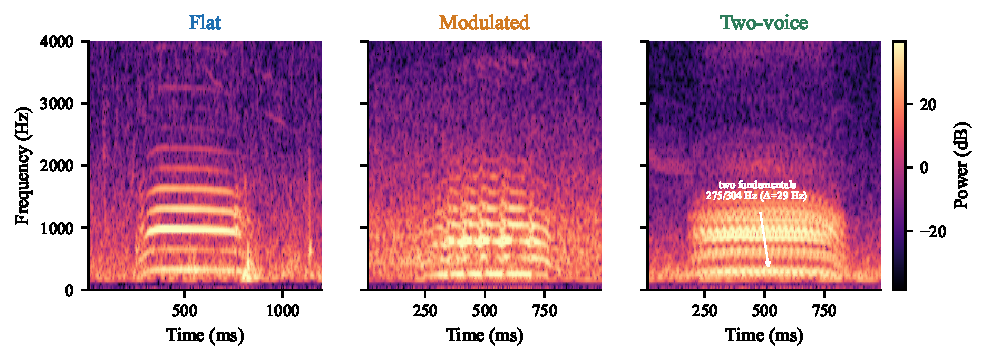
\includegraphics[width=0.92\textwidth]{figures/fig_p1_spectrograms.pdf}
\caption{Spectrograms of representative one-second recordings of the three call types. Flat calls show a stable harmonic stack; modulated calls show frequency modulation and a pulsed temporal structure; two-voice calls show two simultaneous fundamentals. The two fundamentals are only 29 Hz apart, below the 47 Hz spectrogram bin, so they appear as one band; the annotation marks their position.}
\label{fig:spectrograms}
\end{figure}

\begin{figure}[!ht]
\centering
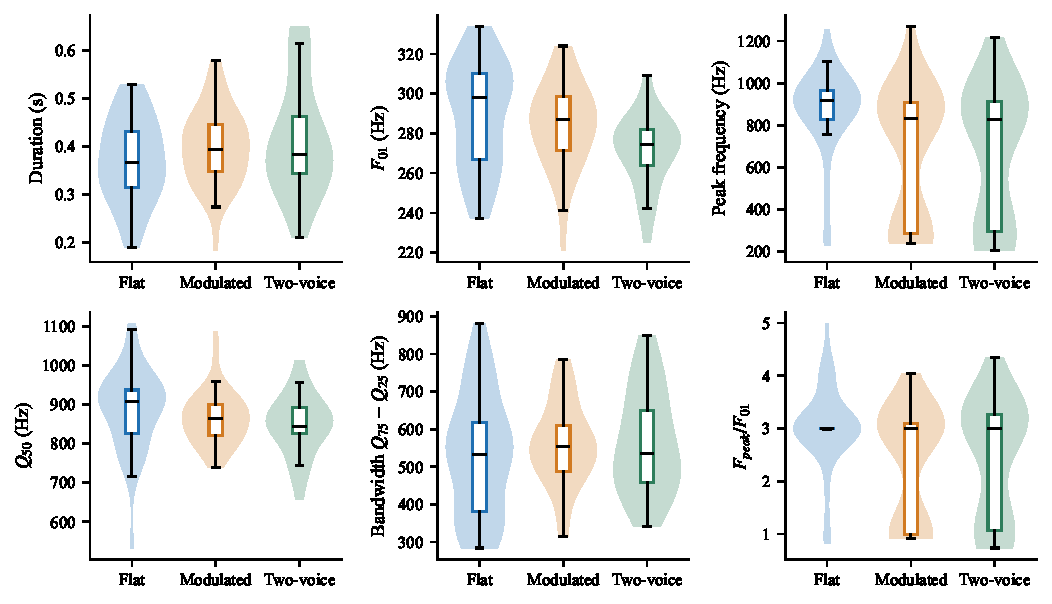
\includegraphics[width=0.92\textwidth]{figures/fig_p1_dist.pdf}
\caption{Distributions of six acoustic measures by call type. Violins show the density, boxes the interquartile range and whiskers the non-outlier range.}
\label{fig:p1dist}
\end{figure}

\subsection{Classification and main influencing factors}

Two caveats frame the accuracy before the models are compared: the overall $93.4\%$ cross-validated accuracy includes definitional identification of two-voice calls, and the pure acoustic discrimination between flat and modulated calls is $73.9\%$.

We compare a multinomial logistic regression with three tree ensembles under repeated stratified five-fold cross-validation (ten repeats, 50 folds). Two feature sets are used. The \emph{reduced} set contains only measures available for every call: duration, $F_{01}$, $F_{\mathrm{peak}}$, $Q_{25}$, $Q_{50}$, $Q_{75}$ and five derived ratios (bandwidth, $F_{\mathrm{peak}}/F_{01}$, $Q_{50}/F_{01}$, $F_{\mathrm{peak}}/Q_{50}$, $Q_{75}/Q_{25}$). The \emph{full} set adds $F_{02}$, pulse rate and two indicators recording whether these structural cues are measurable. Missing values are median-imputed inside the pipeline, and class weights balance the three types. We also evaluate a deployable hierarchical rule: two-voice calls are identified by a measurable $F_{02}$, and flat versus modulated calls are separated by a random forest on the reduced features.

\begin{table}[!ht]
\centering
\caption{Repeated stratified 5-fold cross-validation (10 repeats) for three-class call-type classification.}
\label{tab:p1clf}
\footnotesize
\begin{tabular}{lccc}
\toprule
Model & Accuracy & Balanced accuracy & Macro $F_1$ \\
\midrule
Logistic regression (reduced) & 0.393 $\pm$ 0.079 & 0.390 $\pm$ 0.086 & 0.369 $\pm$ 0.090 \\
Random forest (reduced) & 0.542 $\pm$ 0.108 & 0.529 $\pm$ 0.106 & 0.517 $\pm$ 0.110 \\
Random forest (full) & 0.934 $\pm$ 0.045 & 0.941 $\pm$ 0.040 & 0.942 $\pm$ 0.041 \\
Extra trees (full) & 0.934 $\pm$ 0.043 & 0.941 $\pm$ 0.039 & 0.942 $\pm$ 0.039 \\
Gradient boosting (full) & 0.927 $\pm$ 0.055 & 0.936 $\pm$ 0.048 & 0.936 $\pm$ 0.049 \\
Hierarchical rule + RF & 0.797 $\pm$ 0.070 & 0.817 & 0.817 \\
\bottomrule
\end{tabular}
\par\vspace{2pt}\footnotesize Mean $\pm$ standard deviation over 50 folds. ``Reduced'' uses only universally measured continuous features; ``full'' adds F02, pulse rate and indicators of whether these structural cues are measurable; the hierarchical rule assigns two-voice from the presence of F02 and then separates the other two types with a random forest.
\end{table}

The full random forest reaches $93.4\%$ accuracy (balanced accuracy $94.1\%$, macro $F_1=0.942$), followed closely by extra trees ($93.4\%$) and gradient boosting ($92.7\%$); the reduced random forest reaches only $54.2\%$ and multinomial logistic regression $39.3\%$. The hierarchical rule attains $79.7\%$, of which the second stage (flat versus modulated) contributes $73.9\%$. The confusion matrix in Figure \ref{fig:p1clf} shows that the full model makes only eight errors out of 108: two flat calls are classified as modulated, and six modulated calls as flat; no two-voice call is misclassified.

\begin{figure}[!ht]
\centering
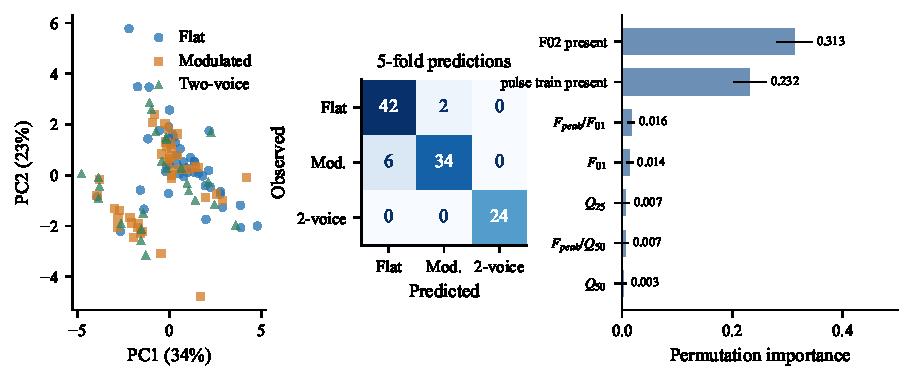
\includegraphics[width=0.92\textwidth]{figures/fig_p1_classifier.pdf}
\caption{Left: principal-component projection of the reduced acoustic features (PC1 and PC2 explain $33.8\%$ and $23.3\%$ of the variance); the overlap of flat and modulated points is the geometric counterpart of the $54.2\%$ reduced-feature accuracy. Centre: cross-validated confusion matrix of the full random forest. Right: permutation importance of the full model.}
\label{fig:p1clf}
\end{figure}

Permutation importance (Appendix Table \ref{tab:p1imp}) explains the gap between the two feature sets. The presence of a second fundamental (importance $0.313$) and of a measurable pulse train ($0.232$) dominate; among continuous measures, $F_{\mathrm{peak}}/F_{01}$ ($0.016$) and $F_{01}$ ($0.014$) contribute most. In the reduced model the leading features are $Q_{50}/F_{01}$ ($0.054$), $F_{01}$ ($0.047$) and $F_{\mathrm{peak}}/F_{01}$ ($0.043$). The three call types are thus not separated by gross spectral envelope but by harmonic and temporal microstructure. This is exactly the structure that propagation is expected to affect differently, and it motivates the representation-specific analysis in Section 4.

\section{Problem 2: Signal Degradation and Effective Range}

\subsection{Composite acoustic fidelity}

For each call type and distance, let $C_{\mathrm{spec}}$, $C_{\mathrm{amp}}$ and $C_{\mathrm{env}}$ be the mean correlations of the spectrogram, amplitude spectrum and envelope with the 1 m reference. Correlations are bounded and heteroscedastic, so we combine them on the Fisher-$z$ scale \cite{fisher1921},
\begin{equation}
F_k(d)=\tanh\!\left(\frac{1}{3}\Bigl[\operatorname{artanh}C_{\mathrm{spec},k}(d)
+\operatorname{artanh}C_{\mathrm{amp},k}(d)
+\operatorname{artanh}C_{\mathrm{env},k}(d)\Bigr]\right).
\label{eq:fidelity}
\end{equation}
The three representations are complementary: the spectrogram encodes frequency modulation over time, the amplitude spectrum encodes the distribution of energy across frequencies, and the envelope encodes the temporal pattern that carries individual identity. Equal weights avoid privileging one representation a priori; Section 4.4 shows that dropping any one representation changes the reliable range by at most a factor of about $1.4$, and that the ranking of call types is unchanged.

\begin{figure}[!ht]
\centering
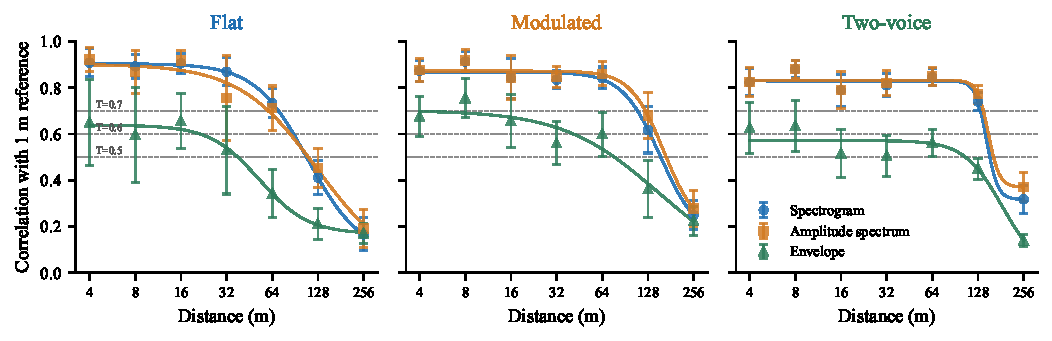
\includegraphics[width=0.92\textwidth]{figures/fig_p2_measures.pdf}
\caption{Correlation with the 1 m reference as a function of distance for the three representations (points: mean $\pm$ standard deviation over 300 replicates; lines: fitted Hill curves; dashed lines: composite fidelity thresholds $T=0.5,0.6,0.7$, shown for reference).}
\label{fig:p2measures}
\end{figure}

\subsection{Degradation model}

Visual inspection (Figure \ref{fig:p2measures}) shows a near-field plateau followed by a sigmoidal decline, which is not captured by a single exponential. We therefore fit the four-parameter Hill decay
\begin{equation}
F_k(d)=F_{\min,k}+\frac{F_{0,k}-F_{\min,k}}{1+(d/d_{h,k})^{\kappa_k}},
\label{eq:hill}
\end{equation}
where $F_{0,k}$ is the near-field fidelity, $F_{\min,k}$ the asymptotic fidelity, $d_{h,k}$ the half-decay distance and $\kappa_k$ the steepness. We compare it with an exponential, a power law and a Weibull decay on all 2{,}100 replicate composite values per call type using AICc \cite{burnham2002}. The Hill and Weibull models have the lowest AICc for all three types and the highest $R^2$ (Appendix Table \ref{tab:p2models}); they are statistically indistinguishable, and we prefer the Hill form because $d_h$ and $\kappa$ have direct interpretations.

The fitted curves (Appendix Table \ref{tab:p2params}) reproduce the observations closely ($R^2=0.968$--$0.994$). Flat calls start highest ($F_0=0.853$) but decay smoothly ($\kappa=1.85$; half-fidelity $101$ m); modulated calls start at $0.823$ and decay more steeply ($\kappa=2.97$; $155$ m); two-voice calls start lowest ($0.766$) but hold a plateau to about $130$ m and then fall sharply ($\kappa=12.0$). At 256 m fidelity is $0.176$, $0.250$ and $0.279$.

\begin{figure}[H]
\centering
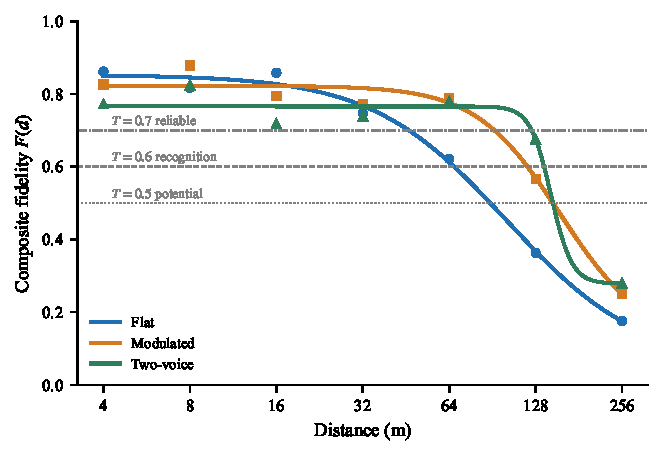
\includegraphics[width=0.62\textwidth]{figures/fig_p2_composite.pdf}
\caption{Composite fidelity $F(d)$ with fitted Hill curves and $90\%$ bootstrap bands. Horizontal lines mark the potential ($0.50$), recognition ($0.60$) and reliable ($0.70$) thresholds.}
\label{fig:p2composite}
\end{figure}

\subsection{Effective ranges at three thresholds}

We interpret the fidelity thresholds ecologically. $T=0.50$ indicates that half of the reference structure remains and is therefore the minimum for \emph{potential recognition}. $T=0.60$ is a working criterion for \emph{recognition}, and $T=0.70$ is a stringent criterion for \emph{reliable recognition} in noise. Solving $F_k(d)=T$ in \eqref{eq:hill} gives
\begin{equation}
d_{T,k}=d_{h,k}\left(\frac{F_{0,k}-T}{T-F_{\min,k}}\right)^{1/\kappa_k}.
\label{eq:range}
\end{equation}
We obtain $95\%$ intervals by resampling the 300 replicates at each distance, refitting the curve and recomputing \eqref{eq:range} 1{,}200 times.

\begin{table}[!ht]
\centering
\caption{Effective communication range (m) for three recognition thresholds; point estimate from the full data and 95\% bootstrap interval in brackets.}
\label{tab:p2ranges}
\small
\begin{tabular}{lccc}
\toprule
Call type & $T=0.50$ (potential) & $T=0.60$ (recognition) & $T=0.70$ (reliable) \\
\midrule
Flat & 89 [88, 90] & 67 [65, 68] & 46 [45, 48] \\
Modulated & 147 [144, 151] & 120 [118, 122] & 92 [89, 95] \\
Two-voice & 147 [146, 148] & 137 [136, 138] & 124 [123, 125] \\
\bottomrule
\end{tabular}
\end{table}

At the potential threshold the ranges are $89$ m (flat), $147$ m (modulated) and $147$ m (two-voice). At the recognition threshold they are $67$, $120$ and $137$ m, and at the reliable threshold $46$, $92$ and $124$ m. Two-voice calls therefore overtake modulated calls as the criterion becomes stricter: their plateau preserves high fidelity to about $130$ m, whereas the smooth decay of modulated calls crosses $0.70$ near $92$ m. Flat calls are consistently the shortest-ranging type. Bootstrap intervals are narrow ($\pm2$ m) because each distance uses 300 replicates; they measure sampling error conditional on the model, not model uncertainty.

\subsection{Sensitivity and robustness}

Three checks probe stability. Varying the threshold from $0.40$ to $0.80$ changes the flat range from $117$ to $24$ m, but the ordering two-voice $>$ modulated $>$ flat holds above $0.55$ (Appendix Table \ref{tab:p2sens}). The decay family matters more: exponential or power-law fits imply reliable ranges of $40$--$60$ m versus $48$--$124$ m for Hill and Weibull, and the exponential cannot reproduce the near-field plateau (Appendix Table \ref{tab:p2mf}). Dropping a representation or using an arithmetic average leaves the ranking unchanged (two-voice reliable range $114$--$136$ m; Appendix Table \ref{tab:p2robust}). Direction is robust; the next subsection quantifies magnitude probabilistically.

\subsection{Hierarchical Bayesian model and probabilistic risk}

The bootstrap intervals of Table \ref{tab:p2ranges} are conditional on the Hill form and on fixed thresholds. Conservation decisions, however, require a predictive statement that integrates parameter uncertainty, threshold ambiguity and noise. We therefore re-estimate the decay hierarchically \cite{gelman2013}. Writing $\theta_k=(F_{0k},F_{\min,k},d_{h,k},\kappa_k)$, we place normal priors on transformed parameters,
\begin{equation}
\operatorname{logit}F_{0k}\sim\mathcal{N}(\mu_{F_0},\tau_{F_0}^2),\qquad
\operatorname{logit}\frac{F_{\min,k}}{F_{0,k}}\sim\mathcal{N}(\mu_{m},\tau_{m}^2),
\label{eq:prior1}
\end{equation}
\begin{equation}
\log d_{h,k}\sim\mathcal{N}(\mu_{d},\tau_{d}^2),\qquad
\log\kappa_k\sim\mathcal{N}(\mu_{\kappa},\tau_{\kappa}^2),
\label{eq:prior2}
\end{equation}
with weakly informative hyperpriors centred on $F_0\approx0.82$, $F_{\min}/F_0\approx0.18$, $d_h\approx120$ m and $\kappa\approx2.5$. The observation model is $F_{k,j}\sim\mathcal{N}(\mathrm{Hill}(d_j;\theta_k),\sigma_k^2)$ on the 2{,}100 composite replicate values per type. Pooling is partial: the hyperprior means are shared, but each call type retains its own parameters, so the shrinkage is strongest for the poorly identified two-voice steepness.

We sample the posterior with an affine-invariant ensemble sampler \cite{foremanmackey2013} using 60 walkers, 2{,}200 iterations, 700 discarded iterations and thinning of 10, which leaves 9{,}000 retained draws at a mean acceptance rate of $0.25$. The posterior medians (Table \ref{tab:p5post}) reproduce the least-squares estimates of Appendix Table \ref{tab:p2params} closely, but the credible intervals are wider and more honest. The near-field fidelity of flat calls is tightly determined ($0.854$ [$0.847$, $0.861$]), whereas the two-voice steepness is right-skewed ($8.55$ [$5.82$, $21.15$]) because the decay is close to a step and $\kappa$ is only weakly identified. The two-voice asymptote ($0.272$ [$0.239$, $0.285$]) is four times that of flat calls ($0.065$ [$0.035$, $0.094$]), which is the parameter-level signature of the plateau.

\begin{table}[!ht]
\centering
\caption{Posterior medians and $95\%$ credible intervals of the Bayesian hierarchical Hill model.}
\label{tab:p5post}
\footnotesize
\begin{tabular}{lccccc}
\toprule
Call type & $F_0$ & $F_{\min}$ & $d_h$ (m) & $\kappa$ & $\sigma$ \\
\midrule
Flat & 0.854 [0.847, 0.861] & 0.065 [0.035, 0.094] & 100 [94, 105] & 1.92 [1.78, 2.06] & 0.083 \\
Modulated & 0.824 [0.819, 0.829] & 0.118 [0.060, 0.173] & 156 [145, 169] & 2.94 [2.62, 3.48] & 0.075 \\
Two-voice & 0.767 [0.763, 0.771] & 0.272 [0.239, 0.285] & 152 [137, 168] & 8.55 [5.82, 21.15] & 0.068 \\
\bottomrule
\end{tabular}
\end{table}

\begin{figure}[!ht]
\centering
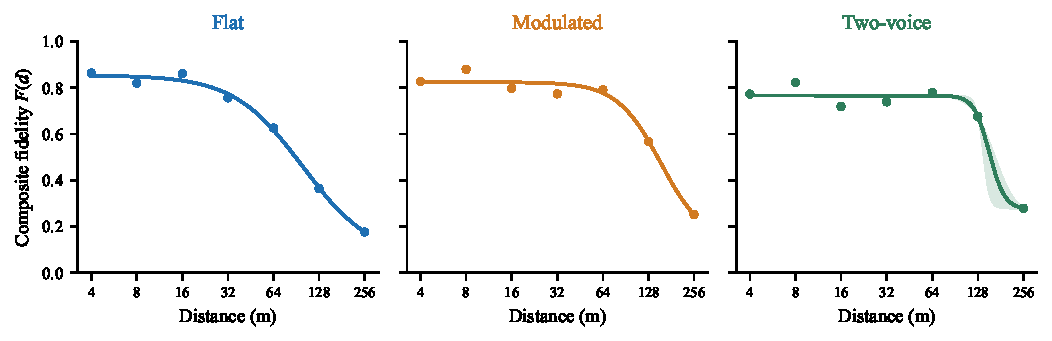
\includegraphics[width=0.88\textwidth]{figures/fig_p5_posterior.pdf}
\caption{Posterior predictive fan charts of the hierarchical Hill model ($90\%$ credible bands) with the observed composite fidelity points.}
\label{fig:p5post}
\end{figure}

To convert the posterior into a risk statement we propagate six concurrent sources of uncertainty in a Monte Carlo simulation. For each of 400 draws we (i) take a posterior draw $\theta^{(s)}$; (ii) draw the recognition threshold $T=0.45+0.30\,\mathrm{Beta}(4,4)$, which has mean $0.60$ and central $90\%$ support close to the conventional $0.50$--$0.70$ range; (iii) draw a proportional correlation loss $\delta=0.20\,\mathrm{Beta}(1.5,4)$, with mean $0.077$ and a heavy right tail representing occasional severe noise; (iv) draw the responder fraction $\phi=0.20+0.60\,\mathrm{Beta}(2,2)$; (v) draw the group size $N$ from its empirical distribution; and (vi) draw the playback coefficients from their cluster-robust multivariate normal. The radius is recomputed from \eqref{eq:radius} with the perturbed fidelity $(1-\delta)F_k(d)$. Because the Hill and Weibull families are indistinguishable by AICc, model-form uncertainty is treated separately in Section 4.6 rather than mixed into these draws.

\begin{table}[!ht]
\centering
\caption{Probabilistic effective radius integrating posterior, threshold, noise, responder-fraction and group-size uncertainty.}
\label{tab:p5risk}
\footnotesize
\begin{tabular}{lccccc}
\toprule
Call type & Radius (m) & $P(r\ge100)$ & $P(r\ge120)$ & $P(r\ge150)$ & $P(r<50)$ \\
\midrule
Flat & 61 [34, 82] & 0 & 0 & 0 & 20 \\
Modulated & 110 [66, 138] & 72 & 30 & 0 & 1 \\
Two-voice & 134 [79, 155] & 96 & 88 & 7 & 2 \\
\bottomrule
\end{tabular}
\end{table}

The predictive distribution is much wider and more asymmetric than the bootstrap intervals (Table \ref{tab:p5risk}). Median radii are $61$ m [$34$, $82$] for flat calls, $110$ m [$66$, $138$] for modulated calls and $134$ m [$79$, $155$] for two-voice calls. The probability that the radius reaches $120$ m is $0\%$ for flat calls, $30\%$ for modulated calls and $88\%$ for two-voice calls, and only two-voice calls have a non-negligible probability ($7\%$) of reaching $150$ m. Flat calls fall below $50$ m in $20\%$ of draws. The point estimates of Section 4.3 ($89$, $147$ and $147$ m) are therefore favourable-scenario medians; in particular, a 100 m flat-call buffer has zero posterior support. Expected responders at 100 m have median $2.1$--$2.3$ but a $95\%$ interval of roughly $0.3$--$12$, because $\phi$ and $N$ are weakly identified.

\begin{figure}[!ht]
\centering
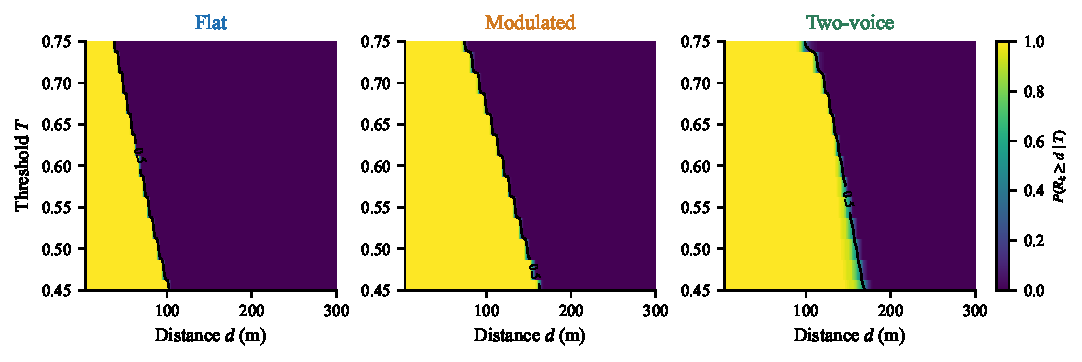
\includegraphics[width=0.92\textwidth]{figures/fig_p5_threshold.pdf}
\caption{Threshold-conditional probability $P(R_k\ge d\mid T)$ of the effective radius from posterior draws; the black contour marks the median ($0.5$).}
\label{fig:p5thr}
\end{figure}

Figure \ref{fig:p5thr} shows where the probability comes from by fixing the threshold. Threshold choice alone moves the two-voice radius: at $T=0.50$ it reaches 150 m with probability $93\%$, at $T=0.60$ it reaches 120 m with probability $100\%$ but 150 m with probability zero, and at $T=0.70$ it still reaches 120 m with probability $85\%$. Modulated calls reach 120 m with probability $63\%$ at $T=0.60$ and never at $T=0.70$, while flat calls never reach 100 m for any threshold in $[0.50,0.75]$. A defensible statement is therefore threshold-specific---``two-voice calls support a 120 m buffer with at least $85\%$ probability for any threshold up to $0.70$''---whereas a universal $100$--$150$ m buffer is not supported.

\subsection{Extrapolation beyond the measured range}

All fits above are interpolations within $4$--$256$ m. Extrapolation is unavoidable in conservation questions about offshore buffers, so we quantify its cost. Table \ref{tab:p5extra} reports the fidelity predicted at $300$ m and $500$ m by the four model families fitted to the same data, and Figure \ref{fig:p5extrap} shows the divergence for two-voice calls. For flat calls the families agree that fidelity is at most $0.17$ at $300$ m and at most $0.16$ at $500$ m, so the qualitative conclusion that flat calls are not recognisable beyond about $250$ m does not depend on the family. For two-voice calls the predicted fidelity at $500$ m ranges from $0.19$ (exponential) to $0.28$ (Hill and Weibull), a factor of $1.5$, and the ordering of the families even reverses between $300$ and $500$ m.

\begin{table}[!ht]
\centering
\caption{Predicted fidelity at 300 m and 500 m by model family, illustrating extrapolation uncertainty beyond the observed 256 m.}
\label{tab:p5extra}
\small
\begin{tabular}{lcccc}
\toprule
Call type & Hill & Weibull & Exponential & Power \\
\midrule
Flat & 0.15 / 0.10 & 0.17 / 0.16 & 0.13 / 0.04 & 0.15 / 0.06 \\
Modulated & 0.21 / 0.14 & 0.24 / 0.24 & 0.27 / 0.12 & 0.29 / 0.15 \\
Two-voice & 0.28 / 0.28 & 0.28 / 0.28 & 0.34 / 0.19 & 0.35 / 0.21 \\
\bottomrule
\end{tabular}
\end{table}

\begin{figure}[!ht]
\centering
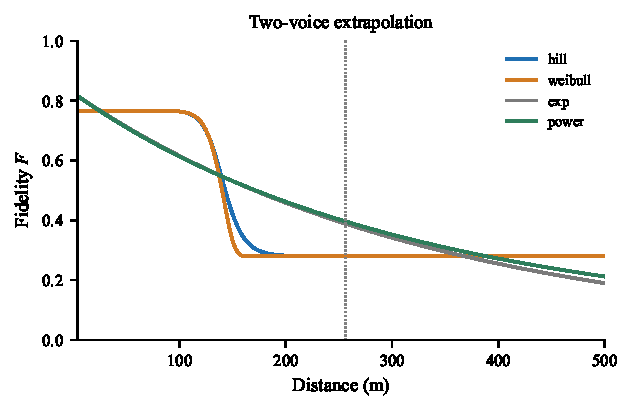
\includegraphics[width=0.55\textwidth]{figures/fig_p5_extrap.pdf}
\caption{Fidelity extrapolated beyond the measured $256$ m by four model families for two-voice calls. The families agree within the data and diverge outside it; predictions beyond $256$ m are not used for management decisions.}
\label{fig:p5extrap}
\end{figure}

Two bounds follow. First, every family places fidelity below the $0.50$ potential-recognition threshold at $300$ m for all three call types, so no model supports communication beyond roughly $300$ m; this is a robust upper bound that can be stated without choosing a family. Second, at $500$ m the plausible fidelity lies in $[0.04,0.28]$, entirely below any recognition criterion, so the precise value is irrelevant to management. We therefore restrict all radius and buffer statements to distances at which the model is supported by data, and we do not extrapolate the effective radius beyond $256$ m. Where a buffer longer than $256$ m is contemplated, the analysis returns ``not quantitatively supported'' rather than a number.

\section{Problem 3: Behavioural Responses to Playback}

\subsection{Response rates and stimulus selectivity}

Table \ref{tab:p3rates} reports response rates. Natural calls elicited any response in $90/139$ trials ($64.7\%$) versus $18/139$ ($12.9\%$) for controls; head-up occurred in $55$ versus $13$ trials, vocalisation in $76$ versus $5$, and approach in $23$ versus $0$. All four differences are significant by two-sided Fisher exact tests ($p<10^{-4}$; Appendix Table \ref{tab:p3fisher}). Among natural calls, two-voice calls have the highest any-response rate ($69.0\%$), followed by modulated ($63.6\%$) and flat ($60.4\%$); vocalisation is highest for two-voice ($58.6\%$), and approach is rare for all types but absent from controls.

\begin{table}[!ht]
\centering
\caption{Observed response rates of playback experiments by stimulus type (count and percentage).}
\label{tab:p3rates}
\small
\begin{tabular}{lrcccc}
\toprule
Stimulus & $N$ & Any response & Head-up & Vocal & Approach \\
\midrule
Control & 139 & 18/139 (12.9\%) & 13/139 (9.4\%) & 5/139 (3.6\%) & 0/139 (0.0\%) \\
Flat & 48 & 29/48 (60.4\%) & 21/48 (43.8\%) & 26/48 (54.2\%) & 4/48 (8.3\%) \\
Modulated & 33 & 21/33 (63.6\%) & 15/33 (45.5\%) & 16/33 (48.5\%) & 8/33 (24.2\%) \\
Two-voice & 58 & 40/58 (69.0\%) & 19/58 (32.8\%) & 34/58 (58.6\%) & 11/58 (19.0\%) \\
All natural calls & 139 & 90/139 (64.7\%) & 55/139 (39.6\%) & 76/139 (54.7\%) & 23/139 (16.5\%) \\
\bottomrule
\end{tabular}
\end{table}

\begin{figure}[!ht]
\centering
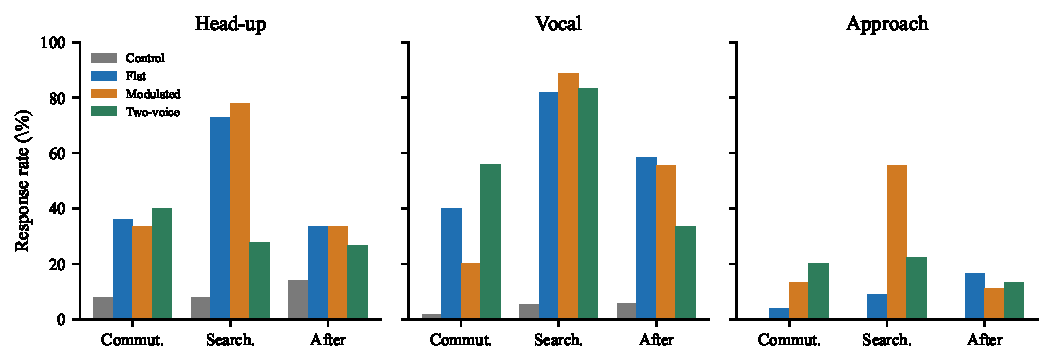
\includegraphics[width=0.92\textwidth]{figures/fig_p3_rates.pdf}
\caption{Response rates by behaviour, call type and context.}
\label{fig:p3rates}
\end{figure}

\subsection{Regression framework}

To separate stimulus, context, distance and group size, we fit cluster-robust logistic regressions with the experiment identifier as the cluster, which accounts for the paired call--control design:
\begin{equation}
\operatorname{logit}\Pr(Y_{i}=1)=\beta_0+\beta_{\mathrm{type}(i)}+\beta_{\mathrm{ctx}(i)}
+\beta_D\log_2 D_i+\beta_N\log_2 N_i .
\label{eq:logit}
\end{equation}
Distance and group size are logged so that coefficients are odds ratios per doubling. Because no control trial elicited approach, the approach model is fitted to natural calls only, with flat as the baseline.

\begin{table}[!ht]
\centering
\caption{Cluster-robust logistic regression of response behaviours on call type, context, distance and group size.}
\label{tab:p3or}
\footnotesize
\begin{tabular}{llccc}
\toprule
Outcome & Contrast & OR & 95\% CI & $p$ \\
\midrule
Any response & Flat vs control & 13.96 & 6.52--29.89 & $<10^{-4}$ \\
Any response & Modulated vs control & 16.16 & 6.32--41.33 & $<10^{-4}$ \\
Any response & Two-voice vs control & 20.86 & 8.70--50.03 & $<10^{-4}$ \\
Any response & Searching vs commuting & 1.91 & 0.72--5.08 & 0.193 \\
Any response & After feeding vs commuting & 1.13 & 0.45--2.82 & 0.794 \\
Any response & Distance (per doubling) & 0.63 & 0.42--0.94 & 0.025 \\
Any response & Group size (per doubling) & 0.70 & 0.53--0.93 & 0.014 \\
Head-up & Flat vs control & 8.48 & 3.70--19.48 & $<10^{-4}$ \\
Head-up & Modulated vs control & 8.64 & 3.43--21.79 & $<10^{-4}$ \\
Head-up & Two-voice vs control & 5.35 & 2.40--11.90 & $<10^{-4}$ \\
Head-up & Searching vs commuting & 1.01 & 0.34--3.05 & 0.981 \\
Head-up & After feeding vs commuting & 0.91 & 0.36--2.29 & 0.846 \\
Head-up & Distance (per doubling) & 0.55 & 0.37--0.82 & 0.0031 \\
Head-up & Group size (per doubling) & 0.77 & 0.57--1.04 & 0.090 \\
Vocal & Flat vs control & 54.98 & 15.68--192.79 & $<10^{-4}$ \\
Vocal & Modulated vs control & 43.10 & 11.62--159.83 & $<10^{-4}$ \\
Vocal & Two-voice vs control & 61.92 & 18.35--208.88 & $<10^{-4}$ \\
Vocal & Searching vs commuting & 2.07 & 0.73--5.85 & 0.169 \\
Vocal & After feeding vs commuting & 1.07 & 0.46--2.47 & 0.871 \\
Vocal & Distance (per doubling) & 1.11 & 0.73--1.70 & 0.622 \\
Vocal & Group size (per doubling) & 0.63 & 0.48--0.84 & 0.0016 \\
Approach (calls only) & Modulated vs flat & 3.57 & 0.93--13.65 & 0.063 \\
Approach (calls only) & Two-voice vs flat & 2.85 & 0.85--9.60 & 0.090 \\
Approach (calls only) & Searching vs commuting & 1.32 & 0.28--6.19 & 0.724 \\
Approach (calls only) & After feeding vs commuting & 0.96 & 0.29--3.16 & 0.940 \\
Approach (calls only) & Distance (per doubling) & 0.62 & 0.38--1.02 & 0.061 \\
Approach (calls only) & Group size (per doubling) & 0.77 & 0.48--1.23 & 0.277 \\
\bottomrule
\end{tabular}
\end{table}

The odds ratios (Table \ref{tab:p3or}) show strong selectivity. Relative to control, flat, modulated and two-voice calls raise the odds of any response by factors of $14.0$, $16.2$ and $20.9$, and the odds of vocalisation by factors of $55$, $43$ and $62$. Distance reduces the odds of any response by a factor of $0.63$ per doubling and of head-up by $0.55$ per doubling, but has no detectable effect on vocalisation ($p=0.62$). Group size reduces the odds of any response ($0.70$ per doubling, $p=0.014$) and of vocalisation ($0.63$, $p=0.002$), but not of head-up or approach. Context effects are small and non-significant after accounting for the other variables. For approach, modulated and two-voice calls have higher odds than flat calls ($3.6$ and $2.9$), but the intervals include one.

The negative group-size effect is counter-intuitive, because larger groups offer more opportunities for at least one individual to respond. Two explanations are compatible: large groups are less cohesive, or a fixed number of responders is a smaller fraction of a large group. Group size is observed rather than assigned, however, and Section 5.5 shows that the effect does not survive a causal audit; we therefore do not interpret it as a dilution mechanism.

\subsection{Response-combination distributions}

The eight possible combinations are unevenly distributed (Appendix Table \ref{tab:p3combo}). Controls are dominated by ``none'' ($87.1\%$), with head-up only ($9.4\%$) and vocal only ($3.6\%$); no control trial produced a multi-modal combination. Natural calls produce a much richer repertoire: vocal only ($20.9\%$), head-up plus vocal ($20.1\%$), head-up plus vocal plus approach ($10.1\%$), vocal plus approach ($3.6\%$) and head-up only ($7.2\%$). A chi-square test on the collapsed five-category table rejects independence of stimulus and combination ($\chi^2=115.3$, permutation $p=0.0005$).

\begin{figure}[!ht]
\centering
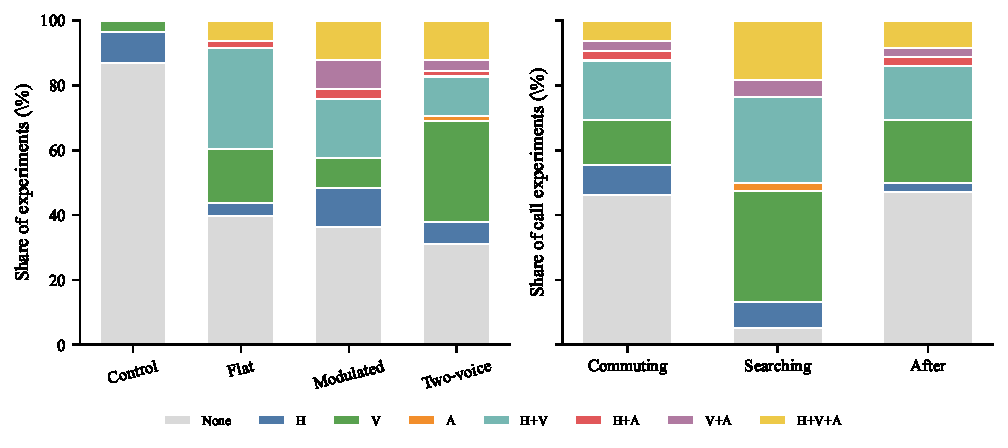
\includegraphics[width=0.92\textwidth]{figures/fig_p3_combos.pdf}
\caption{Composition of response combinations by stimulus (left) and by context for natural calls (right).}
\label{fig:p3combos}
\end{figure}

Within a common multinomial-logit framework,
\begin{equation}
\log\frac{\Pr(C_i=j)}{\Pr(C_i=\text{none})}=\alpha_j+\beta_{j,\mathrm{type}}+\beta_{j,\mathrm{ctx}}
+\beta_{j,D}\log_2D_i+\beta_{j,N}\log_2N_i,
\label{eq:mnlogit}
\end{equation}
call type is the dominant predictor of the outcome distribution. At $N=8$, 50 m and the searching context, the predicted probabilities of ``none'' are $82.8\%$ for control and $26.8\%$, $23.6\%$ and $19.7\%$ for flat, modulated and two-voice calls; the probability of a multi-modal response rises from effectively zero for control to $46.6\%$, $49.1\%$ and $33.6\%$ respectively (Appendix Table \ref{tab:p3combopred}). Two-voice calls instead shift strongly towards vocal-only responses ($38.3\%$). Distance moves probability from multi-modal and vocal-only outcomes towards ``none'', but the call-type ordering is preserved.

\subsection{Latency and intensity}

Response latency is observed only when a behaviour occurs, and a trial without a response is not a missing value but a censored outcome. We therefore use a two-part model. The first part is the logistic occurrence model \eqref{eq:logit}; the second is a log-normal model for the latency of the first overt response among responders,
\begin{equation}
\log(L_i+0.5)\mid Y_i=1 \sim \mathcal{N}\!\left(\gamma_0+\gamma_{\mathrm{type}(i)}
+\gamma_{\mathrm{ctx}(i)}+\gamma_D\log_2D_i+\gamma_N\log_2N_i,\ \sigma^2\right).
\label{eq:latency}
\end{equation}
The model-expected latency, unconditional on response, is
\begin{equation}
\widehat{\mathbb{E}}[L_i]=\widehat{\Pr}(Y_i=1)\,\exp\!\left(\mathbf{x}_i'\widehat{\gamma}+\tfrac12\hat\sigma^2\right).
\label{eq:expLat}
\end{equation}
Intervals are obtained by drawing 4{,}000 coefficient vectors from the cluster-robust covariance and propagating them through \eqref{eq:latency}--\eqref{eq:expLat}.

\begin{table}[!ht]
\centering
\caption{Two-part latency predictions at the median group size ($N=8$) in the searching context; brackets are 95\% simulation intervals from the cluster-robust covariance.}
\label{tab:p3lat}
\footnotesize
\begin{tabular}{llccc}
\toprule
Call type & Distance (m) & P(response) (\%) & Median latency $|$ response (s) & Expected latency (s) \\
\midrule
Control & 50 & 18.1 [7.7, 33.8] & 2.4 [1.5, 3.7] & 0.6 [0.2, 1.3] \\
Control & 100 & 12.3 [4.7, 25.0] & 2.7 [1.6, 4.3] & 0.5 [0.2, 1.0] \\
Control & 150 & 9.8 [3.2, 22.6] & 2.8 [1.7, 4.7] & 0.4 [0.1, 1.0] \\
Flat & 50 & 72.9 [53.3, 87.7] & 2.3 [1.6, 3.4] & 2.4 [1.4, 3.5] \\
Flat & 100 & 63.5 [40.5, 82.8] & 2.6 [1.7, 3.9] & 2.3 [1.2, 3.7] \\
Flat & 150 & 57.2 [32.0, 79.6] & 2.8 [1.8, 4.1] & 2.2 [1.1, 3.7] \\
Modulated & 50 & 75.8 [55.4, 90.1] & 2.2 [1.5, 3.1] & 2.3 [1.4, 3.4] \\
Modulated & 100 & 66.8 [43.4, 84.9] & 2.4 [1.6, 3.6] & 2.2 [1.2, 3.5] \\
Modulated & 150 & 61.2 [36.9, 82.2] & 2.5 [1.7, 3.8] & 2.2 [1.1, 3.5] \\
Two-voice & 50 & 80.1 [63.8, 91.6] & 3.2 [2.0, 4.9] & 3.5 [2.1, 5.5] \\
Two-voice & 100 & 72.2 [53.4, 86.7] & 3.5 [2.3, 5.4] & 3.5 [2.1, 5.5] \\
Two-voice & 150 & 66.5 [44.6, 83.9] & 3.7 [2.4, 5.6] & 3.5 [1.9, 5.5] \\
\bottomrule
\end{tabular}
\end{table}

At $N=8$ in the searching context, the predicted response probability falls from $72.9\%$ to $57.2\%$ for flat calls between 50 and 150 m, from $75.8\%$ to $61.2\%$ for modulated calls and from $80.1\%$ to $66.5\%$ for two-voice calls. Conditional median latencies are short, $2.2$--$3.7$ s, and increase only mildly with distance. Two-voice calls are the slowest ($3.2$--$3.7$ s) but also the most likely to elicit a response; flat and modulated calls are about one second faster. Controls respond less often ($9.8$--$18.1\%$) with similarly short latencies, which confirms that the model is not simply tracking general arousal.

\begin{figure}[!ht]
\centering
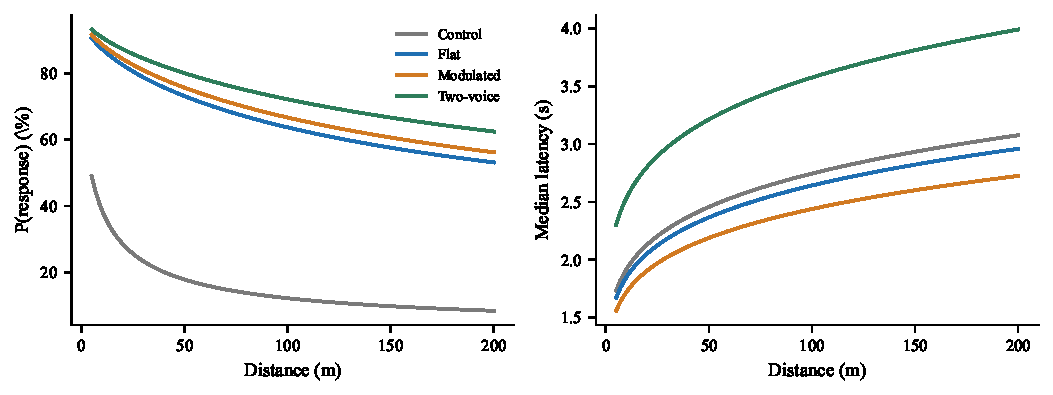
\includegraphics[width=0.92\textwidth]{figures/fig_p3_latency.pdf}
\caption{Predicted response probability (left) and conditional median latency (right) as a function of distance, at $N=8$ and in the searching context.}
\label{fig:p3latency}
\end{figure}

The same hurdle logic describes response intensity (Appendix Table \ref{tab:p3int}). At 100 m, modulated calls yield the highest expected head-up duration ($9.1$ s) and approach duration ($7.1$ s), two-voice calls yield the highest vocal count ($2.7$) and the longest approach duration conditional on approach ($46.1$ s), and flat calls yield the lowest expected values for all three. These patterns are consistent with the fidelity ranking: the calls that retain structure at distance also elicit more intense behaviour.

\subsection{Causal caution: confounding, sensitivity and negative control}

The regressions in Section 5.2 are associational: call type is assigned, but distance, group size, context and sea state are observed, and pairing removes only the call--control contrast. For an odds ratio, the E-value is the minimum strength of association that an unmeasured confounder would need with both the exposure and the outcome, on the risk-ratio scale, to move the estimate to the null \cite{vanderweele2017}. With the common-outcome approximation $\mathrm{RR}\approx\sqrt{\mathrm{OR}}$, the E-values are $6.9$, $7.5$ and $8.6$ for the flat, modulated and two-voice contrasts, and $1.8$ and $1.7$ for distance and group size (Table \ref{tab:p6evalue}).

\begin{table}[!ht]
\centering
\caption{E-values for the main playback effects: the minimum strength of association that an unmeasured confounder would need with both exposure and outcome to explain away the estimate.}
\label{tab:p6evalue}
\small
\begin{tabular}{lccc}
\toprule
Contrast & Odds ratio & E-value & Robustness \\
\midrule
Flat vs control & 13.96 & 6.93 & robust \\
Modulated vs control & 16.19 & 7.51 & robust \\
Two-voice vs control & 20.92 & 8.62 & robust \\
Distance (per doubling) & 0.63 & 1.83 & fragile \\
Group size (per doubling) & 0.70 & 1.68 & fragile \\
\bottomrule
\end{tabular}
\end{table}

The asymmetry is the point. Explaining away the flat-call effect would require a confounder with risk ratio at least $6.9$ with both call type and response, which is implausible; the distance and group-size effects are fragile, since a confounder with risk ratio about $1.7$ could eliminate them, and the distance gradient may partly reflect the conditions of distant trials.

We examine group size directly by dichotomising $N>8$ and estimating the marginal odds ratio by inverse propensity weighting. The propensity score $\Pr(\text{large}\mid\text{call type},\text{context},\text{distance})$ is estimated by logistic regression \cite{rosenbaum1983}, weights are stabilised and trimmed at the first and ninety-ninth percentiles, and intervals come from a 400-replicate cluster bootstrap. The crude odds ratio of $0.49$ ($0.30$--$0.80$) attenuates to $0.51$ ($0.24$--$1.05$) after adjustment and to $0.76$ ($0.39$--$1.48$) under weighting; in control trials, where no call is played, the negative-control odds ratio is $0.93$ ($0.62$--$1.37$) (Table \ref{tab:p6ipw}). The negative effect is thus not identified: once selection into large groups is accounted for, the data are compatible with no effect.

\begin{table}[!ht]
\centering
\caption{Effect of belonging to a large group ($N>8$) on any response: crude, covariate-adjusted, inverse-propensity-weighted, and a control-only negative-control test.}
\label{tab:p6ipw}
\small
\begin{tabular}{lcc}
\toprule
Model & OR (large vs small group) & 95\% CI \\
\midrule
Crude & 0.49 & 0.30--0.80 \\
Adjusted & 0.51 & 0.24--1.05 \\
IPW (marginal) & 0.76 & 0.39--1.48 \\
Control trials only & 0.93 & 0.62--1.37 \\
\bottomrule
\end{tabular}
\end{table}

Covariate balance is adequate: the largest absolute standardised mean difference falls from $1.14$ to $0.07$ after weighting (Appendix Table \ref{tab:p6smd}), and the propensity-score distributions overlap in the two groups.

We therefore treat group size as a descriptor of trial conditions rather than a causal lever, and we do not use it to justify a management action. The same caution applies to the distance coefficient when it is read as a causal effect of distance rather than as a description of the trials. All conservation statements below are phrased conditionally on the call type and on the acoustic model, which are the components that survive the audit.

\subsection{Conditional response decomposition}

The combination analysis treats the eight outcomes as cross-sectional. A finer question is conditional: given that a bird has already raised its head, how likely is it to vocalise, and given vocalisation, to approach? We fit three logistic models on nested subsets with the same cluster-robust specification: head-up on all trials, vocalisation among trials with head-up, and approach among natural-call trials with vocalisation. The product $P(H)\,P(V\mid H)\,P(A\mid V)$ is the joint probability of the three responses, reported at 100 m, $N=8$ and the searching context in Table \ref{tab:p6casc} and Figure \ref{fig:p6cascade}.

\begin{table}[!ht]
\centering
\caption{Conditional response probabilities at 100 m, $N=8$, searching context (percentages); the last column is the product of the three, not a time-stamped sequence.}
\label{tab:p6casc}
\small
\begin{tabular}{lcccc}
\toprule
Call type & $P(H)$ & $P(V\mid H)$ & $P(A\mid V)$ & $P(H,V,A)$ \\
\midrule
Control & 5.8 & 0.0 & 0.0 & 0.0 \\
Flat & 34.3 & 94.6 & 9.7 & 3.2 \\
Modulated & 34.7 & 82.3 & 37.5 & 10.7 \\
Two-voice & 24.7 & 86.0 & 23.9 & 5.1 \\
\bottomrule
\end{tabular}
\end{table}

\begin{figure}[!ht]
\centering
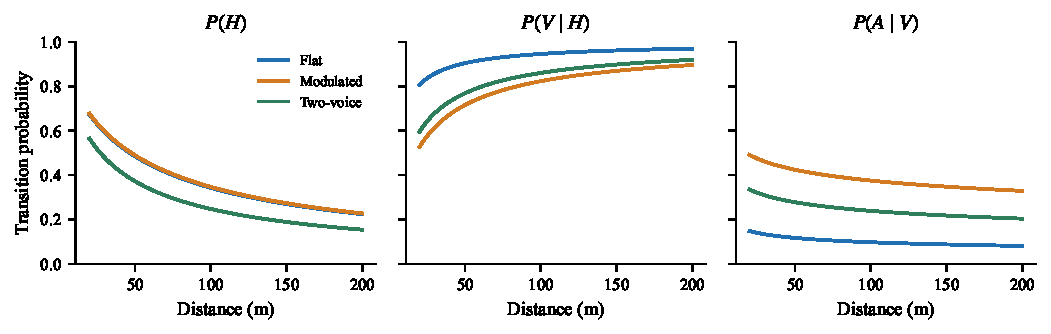
\includegraphics[width=0.92\textwidth]{figures/fig_p6_cascade.pdf}
\caption{Cross-sectional conditional probabilities $P(H)$, $P(V\mid H)$ and $P(A\mid V)$ as functions of distance for the three call types; the sequence is not a proven temporal order.}
\label{fig:p6cascade}
\end{figure}

The decomposition exposes a contrast that marginal response rates conceal. All three types initiate head-up at similar rates ($24.7$--$34.7\%$). Conditional on head-up, flat calls vocalise with probability $94.6\%$, but conditional on vocalisation they approach with only $9.7\%$, so the joint probability is $3.2\%$. Modulated calls vocalise less often after head-up ($82.3\%$) but approach far more often ($37.5\%$), giving the highest joint probability ($10.7\%$); two-voice calls are intermediate ($5.1\%$). The call types therefore differ less in whether they attract attention than in whether attention is accompanied by approach, which is consistent with a contact or alert function for flat calls and a recruitment function for modulated calls. It also explains why the effectiveness ranking changes when approach, rather than any response, is the target.

The decomposition is cross-sectional, not a demonstrated temporal sequence: behaviours were recorded as separate binary outcomes, not time-stamped states, and vocalisation can occur without a preceding head-up. A continuous-time Markov model with observed transition times would be needed to identify transition rates.

\section{Problem 4: Communication-Effectiveness Index and Radii}

\subsection{Index definition}

A call is ecologically effective only if it is both recognisable and answered. We therefore combine the two components multiplicatively:
\begin{equation}
I_k(d)=\bigl[F_k(d)\bigr]^{1/2}\bigl[P_k(d)\bigr]^{1/2},
\label{eq:index}
\end{equation}
where $F_k(d)$ is the fidelity from \eqref{eq:hill} and $P_k(d)$ is the group response probability from \eqref{eq:logit} evaluated at the median group size $N=8$ and the searching context. The exponents $1/2$ give signal availability and behavioural response equal weight and make $I$ the geometric mean of the two. The geometric form preserves the zero limit of a limiting-factor law---if either component vanishes the index vanishes---but, unlike $\min(F,P)$, it permits finite compensation, so a strong component can partly offset a weaker one; it is a symmetric, scale-free composite rather than a strict bottleneck. Because $I$ is dimensionless and bounded by one, it can be compared across call types, distances and scenarios.

The role of the index must be stated precisely. In the observed range fidelity is the binding constraint: wherever $F_k(d)=T=0.50$, the response probability already exceeds $0.5$ (Table \ref{tab:p4comp}), so $I=\sqrt{FP}>0.5$ and the condition $I\ge I^{\ast}$ is inactive. The operational radius is therefore set by $F\ge T$, and the independent contribution of the index lies in the low-fidelity, high-response region: the distance $d_I$ at which $I=0.5$ exceeds the fidelity radius $d_F$ by $27$, $24$ and $15$ m for flat, modulated and two-voice calls (Appendix Table \ref{tab:p4weights}). This difference measures how far a call remains behaviourally effective after it has lost half of its structure, and it is the quantity that the composite index contributes rather than a re-scaling of the fidelity radius.

The expected number of individuals responding to one stimulus is
\begin{equation}
E_k(d)=N\,\phi\,P_k(d),
\label{eq:responders}
\end{equation}
where $\phi$ is the proportion of group members that respond when the group responds. The data record group-level outcomes only, so $\phi$ is not identified; we adopt $\phi=0.5$ as a baseline and report $0.25$ and $0.75$ as sensitivity scenarios.

\subsection{Effective radius}

We define the effective communication radius as the largest distance at which the signal is still recognisable and the index remains at least $0.5$:
\begin{equation}
r_k=\max\left\{d:\ F_k(d)\ge T,\ I_k(d)\ge I^{\ast}\right\},
\qquad T=0.50,\quad I^{\ast}=0.50 .
\label{eq:radius}
\end{equation}
The fidelity condition is the operative one in the observed range: it prevents a high response probability from compensating for a signal that has already lost half of its structure. The index condition is retained as a safeguard against a recognisable but behaviourally ineffective signal, and Section 6.2 shows that at $I^{\ast}=0.5$ it is inactive. Both conditions are evaluated on a fine grid and refined by Brent root finding.

\begin{table}[!ht]
\centering
\caption{Components of the communication-effectiveness index for a typical group ($N=8$, $\phi=0.5$, searching context).}
\label{tab:p4comp}
\small
\begin{tabular}{llcccc}
\toprule
Call type & Distance (m) & Fidelity $F$ & P(response) & Index $I$ & Expected responders \\
\midrule
Flat & 50 & 0.682 & 0.742 & 0.711 & 2.97 \\
Flat & 100 & 0.457 & 0.644 & 0.542 & 2.58 \\
Flat & 150 & 0.313 & 0.580 & 0.426 & 2.32 \\
Modulated & 50 & 0.799 & 0.769 & 0.784 & 3.07 \\
Modulated & 100 & 0.673 & 0.677 & 0.675 & 2.71 \\
Modulated & 150 & 0.489 & 0.615 & 0.549 & 2.46 \\
Two-voice & 50 & 0.766 & 0.811 & 0.788 & 3.24 \\
Two-voice & 100 & 0.760 & 0.730 & 0.745 & 2.92 \\
Two-voice & 150 & 0.470 & 0.674 & 0.563 & 2.69 \\
\bottomrule
\end{tabular}
\end{table}

The component table shows where the limitation lies. At 50 m the index is $0.71$--$0.79$ and the expected number of responders is $3.0$--$3.2$ out of four (expectations assume $\phi=0.5$; at 100 m the range across $\phi=0.25$--$0.75$ is $1.3$--$4.4$, Appendix Table \ref{tab:p4phi}); at 150 m the index falls to $0.43$--$0.56$ and responders to $2.3$--$2.7$. Fidelity, not response probability, is the binding constraint at long range: response probability remains above $0.57$ at 150 m, while fidelity falls to $0.31$--$0.49$. This asymmetry is the quantitative justification for treating signal degradation, rather than motivation, as the primary limit on communication range.

\begin{figure}[!ht]
\centering
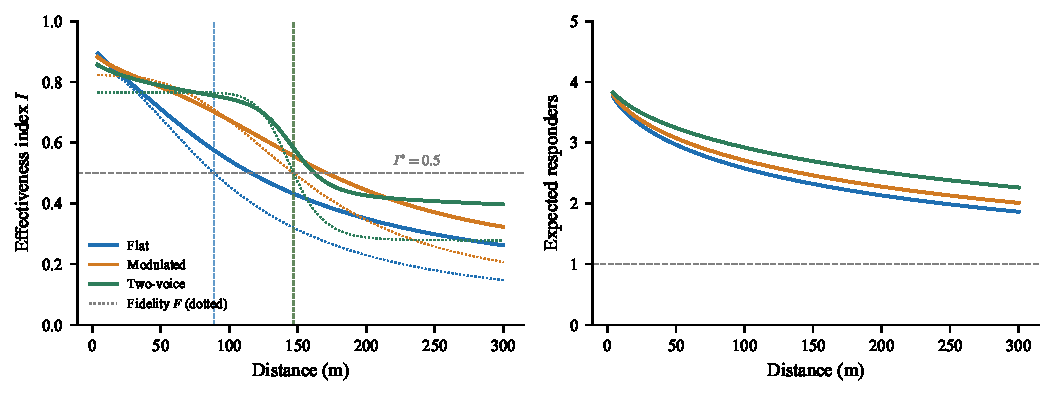
\includegraphics[width=0.92\textwidth]{figures/fig_p4_index.pdf}
\caption{Left: communication-effectiveness index $I(d)$ (solid), fidelity $F(d)$ (dotted) and the operational radius (vertical dashed line, where $F$ falls below $T$). Right: expected number of responding individuals at $N=8$ and $\phi=0.5$.}
\label{fig:p4index}
\end{figure}

\begin{table}[!ht]
\centering
\caption{Effective communication radius (m): the largest distance satisfying both $I\ge0.50$ and $F\ge T$, under the baseline and five degradation scenarios.}
\label{tab:p4radius}
\small
\begin{tabular}{lcccccc}
\toprule
Call type & Baseline & $T=0.60$ & $T=0.70$ & $-10\%$ & $-20\%$ & $-10\%$, $T=0.60$ \\
\midrule
Flat & 89 & 67 & 46 & 76 & 61 & 53 \\
Modulated & 147 & 120 & 92 & 132 & 113 & 102 \\
Two-voice & 147 & 137 & 124 & 141 & 134 & 129 \\
\bottomrule
\end{tabular}
\end{table}

The baseline radii are $89$ m for flat calls, $147$ m for modulated calls and $147$ m for two-voice calls (Table \ref{tab:p4radius}). The equality of the latter two reflects their fitted Hill curves crossing $0.50$ at the same distance, not an index trade-off: as shown below, fidelity alone determines the radius in this range. Under a strict recognition threshold ($T=0.70$), the radii become $46$, $92$ and $124$ m, and two-voice calls are clearly superior.

The weight grid makes the composite's role explicit. Varying $\alpha$ from $0$ (response only) through $0.5$ to $1$ (fidelity only) changes the index crossing $d_I$ from $244$--$400$ m at $\alpha=0$ to $89$--$147$ m at $\alpha=1$ (Appendix Table \ref{tab:p4weights}), but in every case $d_I>d_F$, so the operational radius $\min(d_F,d_I)$ equals $d_F$ and the ordering of call types is unchanged. The result is therefore not an artefact of equal weighting: the geometric mean is conservative relative to response-only or fidelity-only forms, and its independent information is the gap $d_I-d_F$ rather than the radius itself.

\subsection{Noise and sensitivity scenarios}

We model increased ambient noise or adverse sea state as a uniform proportional loss $\delta$ of correlation at all distances, $F_k^{\delta}(d)=(1-\delta)F_k(d)$, optionally combined with a stricter threshold. This is a conservative representation: it reduces fidelity without changing the shape of the decay or the behavioural response, so it isolates the acoustic channel.

\begin{figure}[!ht]
\centering
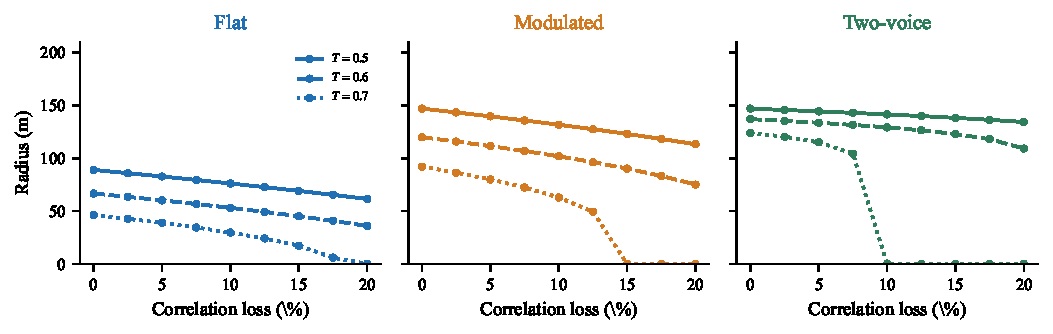
\includegraphics[width=0.92\textwidth]{figures/fig_p4_heatmap.pdf}
\caption{Effective radius as a function of correlation loss for three recognition thresholds. Curves terminate where the near-field fidelity falls below the threshold.}
\label{fig:p4noise}
\end{figure}

A $10\%$ loss reduces the baseline radii to $76$, $132$ and $141$ m; a $20\%$ loss reduces them to $61$, $113$ and $134$ m (Figure \ref{fig:p4noise}). The ordering changes in an ecologically meaningful way: under a $20\%$ loss, two-voice calls (formerly tied with modulated calls) are $21$ m ahead, because their plateau is more robust to a proportional reduction. Combining a $10\%$ loss with the recognition threshold of $0.60$ yields $53$, $102$ and $129$ m. The interaction with the stringent $0.70$ threshold is highly non-linear: a $10\%$ loss leaves only about $30$ m for flat calls and $63$ m for modulated calls, and eliminates reliable recognition for two-voice calls altogether, because their near-field fidelity ($0.766$) falls below $0.70/0.90=0.778$ (Figure \ref{fig:p4noise}). Reliable recognition at $0.70$ therefore has very little headroom under additional noise, which is an argument for treating $0.60$ as the operational criterion.

Sensitivity to $\phi$ is linear (Appendix Table \ref{tab:p4phi}): at 100 m and $N=8$, expected responders are $2.6$--$2.9$ at $\phi=0.5$ and $1.3$--$1.5$ at $\phi=0.25$. Group size is also near-linear: $N=3$ to $20$ raises responders from $1.1$--$1.2$ to $5.3$--$6.3$ (Appendix Table \ref{tab:p4group}). The radius is independent of $\phi$ and only weakly dependent on $N$.

\subsection{Conservation implications}

The results support four conditional management recommendations. First, at the point estimates a precautionary acoustic buffer of $100$--$150$ m around actively vocalising groups protects the range within which two-voice and modulated calls remain recognisable, but the probabilistic analysis qualifies the number: a $100$ m buffer is supported with probability $96\%$ for two-voice calls, $72\%$ for modulated calls and $0\%$ for flat calls. A single buffer therefore cannot be justified for all call types. This scale is broadly consistent with the avoidance responses to anthropogenic sound at comparable distances reported by Pichegru et al. \cite{pichegru2017}. Second, two-voice calls are the appropriate focus of passive acoustic monitoring because they retain information furthest. Third, noise management should target the $250$--$950$ Hz band, where the three types differ most; narrow-band masking there is disproportionately harmful. Fourth, because the negative group-size effect did not survive the causal audit, we do not recommend changing protocols on its basis; group composition and spacing should still be recorded as candidate confounders. Playback evidence is associational (Section 5.2), though call-type effects survive Section 5.5; the radii rest on the propagation model rather than on the regression.

The analysis also suggests three improvements for future playback studies: measure pulse rate on flat calls so that the reduced classifier is not handicapped by structurally missing features; record individual identities, behaviour order and repeated responses with time stamps so that $\phi$ and the response decomposition can be estimated rather than assumed; and log ambient noise and sea state at the trial location so that the correlation-loss distribution can be calibrated rather than hypothesised.

\subsection{Constrained buffer allocation}

A single radius for every colony is inefficient when zones differ in call-type mix and noise. We therefore formulate buffer planning as a constrained optimisation \cite{boyd2004}. Consider three illustrative zones: zone A is flat-call dominated and noisy ($\mathbf{w}_A=(0.6,0.3,0.1)$, $\delta_A=0.15$), zone B is mixed ($\mathbf{w}_B=(0.3,0.4,0.3)$, $\delta_B=0.10$) and zone C is two-voice dominated and quiet ($\mathbf{w}_C=(0.1,0.3,0.6)$, $\delta_C=0.05$). Here $w_{ik}$ is the share of call type $k$ in zone $i$ and $\delta_i$ is the proportional correlation loss. For a buffer of radius $r_i$ in zone $i$, the weighted coverage is the average probability that a call is still within its effective radius anywhere inside the buffer,
\begin{equation}
C_i(r_i)=\sum_{k} w_{ik}\,\frac{1}{r_i-4}\int_{4}^{r_i}S_k(x\mid\delta_i)\,dx,
\label{eq:coverage}
\end{equation}
where $S_k(x\mid\delta_i)=\Pr(R_k\ge x)$ is the posterior survival curve of the effective radius under noise $\delta_i$, obtained from the Bayesian draws of Section 4.5. Averaging over the buffer, rather than evaluating only at its edge, reflects the fact that communication occurs throughout the protected area.

The planning problem is
\begin{equation}
\max_{r_A,r_B,r_C}\ \sum_{i\in\{A,B,C\}}C_i(r_i)
\quad\text{subject to}\quad \sum_i c_i r_i\le B,\qquad 10\le r_i\le 200,
\label{eq:bufferopt}
\end{equation}
where $B$ is the total buffer budget in metres and $c_i$ is the cost per metre, set to one for equal-cost zones. The problem is smooth and low-dimensional, and we solve it by sequential least squares with multiple random starts to avoid local optima.

\begin{table}[!ht]
\centering
\caption{Constrained buffer allocation: optimal zone-specific radii, total weighted coverage, and comparison with a uniform radius policy.}
\label{tab:p7opt}
\small
\begin{tabular}{lcccccc}
\toprule
Budget $B$ (m) & $r_A$ & $r_B$ & $r_C$ & Optimal coverage & Uniform coverage & Gain (\%) \\
\midrule
90 & 30 & 30 & 30 & 2.308 & 2.308 & 0.0 \\
120 & 40 & 40 & 40 & 2.500 & 2.500 & 0.0 \\
150 & 45 & 52 & 53 & 2.606 & 2.565 & 1.6 \\
180 & 46 & 54 & 80 & 2.631 & 2.505 & 5.0 \\
210 & 46 & 54 & 108 & 2.632 & 2.431 & 8.3 \\
240 & 46 & 54 & 108 & 2.632 & 2.374 & 10.8 \\
\bottomrule
\end{tabular}
\end{table}

\begin{figure}[!ht]
\centering
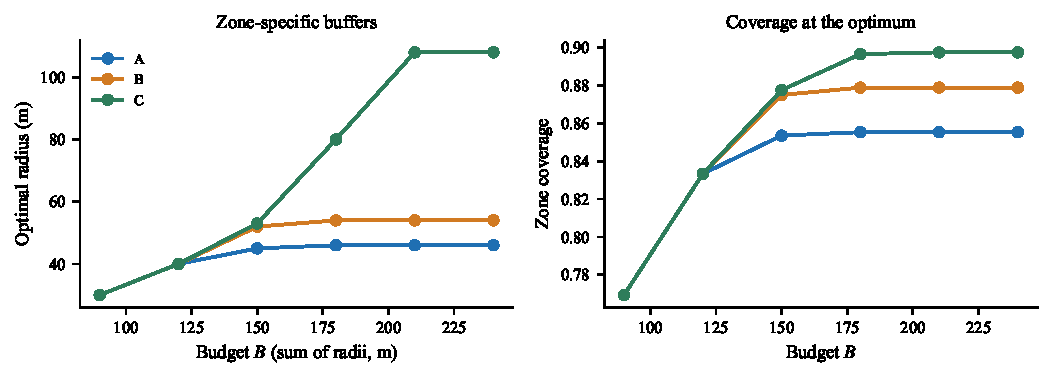
\includegraphics[width=0.92\textwidth]{figures/fig_p7_opt.pdf}
\caption{Left: optimal zone-specific buffer radii as a function of the total budget. Right: weighted coverage attained in each zone at the optimum.}
\label{fig:p7opt}
\end{figure}

For budgets up to $120$ m the constraint binds and the optimal policy is uniform, because every additional metre still buys coverage in all three zones (Table \ref{tab:p7opt}). From $B=150$ m the optimum becomes spatially selective: it stops at about $46$ m in zone A, $52$--$54$ m in zone B and directs the remaining budget to zone C, reaching $108$ m there at $B=210$--$240$ m. Relative to the best uniform policy the coverage gain is $1.6\%$ at $B=150$, $5.0\%$ at $B=180$, $8.3\%$ at $B=210$ and $10.8\%$ at $B=240$ (Figure \ref{fig:p7opt}). The mechanism is that flat-call recognition is already near zero beyond about $50$ m in the noisy zone, while the quiet two-voice zone is still productive at $100$ m. Perturbing each zone weight by $\pm20\%$ and the noise by $\pm0.03$--$0.05$ (approximately $\pm3$ dB in the fitted decay) leaves the call-type ranking invariant (two-voice $>$ modulated $>$ flat; Appendix Table \ref{tab:p7rank}), preserves $r_C>r_B>r_A$ and keeps the gain positive ($8.3$--$14.1\%$ at $B=240$; Appendix Table \ref{tab:p7sens}); the qualitative ranking is thus invariant to plausible perturbations of the illustrative inputs.

This turns the verbal ``$100$--$150$ m buffer'' into a budget-dependent rule: a tight budget protects the quiet two-voice zone first, while a generous budget saturates near $46$, $54$ and $108$ m. With mapped composition, measured noise fields and real costs, \eqref{eq:coverage}--\eqref{eq:bufferopt} become a site-specific tool.

\section{Model Evaluation}

\subsection{Strengths}

The analysis has four strengths. It is \emph{end-to-end}: the same call types are followed from acoustic structure through propagation to behaviour and to a range estimate, so the assumptions linking the stages are explicit. It is \emph{probabilistic}: a hierarchical Bayesian model and a joint Monte Carlo propagate parameter, threshold, noise, responder-fraction and group-size uncertainty, so the output is a distribution of effective radii rather than a single curve. It is \emph{causally audited}: E-values, inverse-propensity weighting and a negative-control test separate the effects that survive confounding from those that do not, and the conservation language is calibrated to that distinction. Finally, it is \emph{actionable}: the constrained buffer optimisation converts the estimates into a budget-dependent spatial allocation rule, and all analyses are scripted in Python with fixed seeds so that the results are reproducible (Appendix \ref{app:code}).

\subsection{Weaknesses}

Five limitations should be acknowledged. First, correlation with a 1 m reference is a proxy for recognition, not a measure of discriminability; thresholds are conventions, and although their uncertainty is propagated, the prior over $T$ and the hyperprior widths are judgements, and future work should vary the latter to assess posterior stability. Second, the propagation measurements cover seven distances and 300 replicates, enough to estimate the mean curve precisely but not to resolve site-specific effects, and we refuse to extrapolate radii beyond $256$ m. Third, the playback data are group-level and observational; the causal audit shows that the call-type effects are robust, but the distance and group-size effects are not, and no analysis of observational data can rule out every confounder. Fourth, the response decomposition is cross-sectional because the behaviours were not time-stamped, so the transition interpretation remains a hypothesis. Fifth, the buffer zones, weights and costs are illustrative; the optimisation demonstrates the method rather than prescribing radii for a particular colony, and the input sensitivity in Section 6.5 supports only the ordering, not the exact gain.

\subsection{Extensions}

Three extensions would strengthen the chain. A transmission experiment with individually identified calls and receivers would replace the correlation proxy with a discrimination measure and would allow the threshold prior to be estimated rather than elicited. A continuous-time multi-state Markov model fitted to time-stamped playback responses would identify transition rates and test the decomposition hypothesis directly. Coupling \eqref{eq:coverage} with a mapped noise field and measured exclusion costs would turn the illustrative zones into a site-specific conservation plan. A receiver-operating-characteristic analysis using playback responses as labels could also estimate the recognition threshold directly, and the representation weights could be fitted from behaviour; we retain conventional thresholds and equal weights because both would be weakly identified with 278 trials.

\section{Conclusion}

Our probabilistic end-to-end pipeline yields several robust findings. First, the three African penguin call types are distinguished mainly by harmonic--temporal microstructure rather than by gross spectral envelope: a full-cue classifier reaches $93.4\%$, but a model restricted to universally measured spectral summaries reaches only $54.2\%$. Second, two-voice calls show a counter-intuitive long-range advantage: despite lower near-field fidelity, their plateau-shaped Hill decay delays collapse, giving predictive radii of $61$, $110$ and $134$ m and probabilities of $0\%$, $30\%$ and $88\%$ of reaching $120$ m. Third, playback experiments confirm robust call-type effects after causal sensitivity audit, whereas the negative group-size association cannot be interpreted as causal; the conditional response decomposition shows that call types differ less in attracting attention than in whether attention is accompanied by approach. Fourth, constrained buffer optimisation yields a budget-dependent allocation rule that protects the quiet two-voice zone first, and its qualitative ranking is invariant to plausible perturbations of the illustrative inputs. Limitations and future directions are discussed in Sections 7.2--7.3.

\begingroup
\scriptsize
\begin{thebibliography}{24}

\bibitem{iucn2024} IUCN SSC Penguin Specialist Group. \textit{Spheniscus demersus}. The IUCN Red List of Threatened Species, 2024.

\bibitem{aubin2002} Aubin T, Jouventin P. How to vocally identify kin in a crowd: the penguin model[J]. Advances in the Study of Behavior, 2002, 31: 243--277.

\bibitem{favaro2014} Favaro L, Ozella L, Pessani D. The vocal repertoire of the African penguin (\textit{Spheniscus demersus}): structure and function of calls[J]. PLoS ONE, 2014, 9(7): e103460.

\bibitem{favaro2015} Favaro L, Gamba M, Alfieri C, Pessani D, McElligott A G. Vocal individuality cues in the African penguin (\textit{Spheniscus demersus}): a source--filter theory approach[J]. Scientific Reports, 2015, 5: 17255.

\bibitem{wiley1978} Wiley R H, Richards D G. Physical constraints on acoustic communication in the atmosphere: implications for the evolution of animal vocalizations[J]. Behavioral Ecology and Sociobiology, 1978, 3: 69--94.

\bibitem{forrest1994} Forrest T G. From sender to receiver: propagation and environmental effects on acoustic signals[J]. American Zoologist, 1994, 34: 644--654.

\bibitem{kruskal1952} Kruskal W H, Wallis W A. Use of ranks in one-criterion variance analysis[J]. Journal of the American Statistical Association, 1952, 47: 583--621.

\bibitem{holm1979} Holm S. A simple sequentially rejective multiple test procedure[J]. Scandinavian Journal of Statistics, 1979, 6: 65--70.

\bibitem{fisher1921} Fisher R A. On the ``probable error'' of a coefficient of correlation deduced from a small sample[J]. Metron, 1921, 1: 3--32.

\bibitem{burnham2002} Burnham K P, Anderson D R. Model Selection and Multimodel Inference: A Practical Information-Theoretic Approach[M]. 2nd ed. New York: Springer, 2002.

\bibitem{gelman2013} Gelman A, Carlin J B, Stern H S, Dunson D B, Vehtari A, Rubin D B. Bayesian Data Analysis[M]. 3rd ed. Boca Raton: CRC Press, 2013.

\bibitem{foremanmackey2013} Foreman-Mackey D, Hogg D W, Lang D, Goodman J. emcee: the MCMC hammer[J]. Publications of the Astronomical Society of the Pacific, 2013, 125: 306--312.

\bibitem{vanderweele2017} VanderWeele T J, Ding P. Sensitivity analysis in observational research: introducing the E-value[J]. Annals of Internal Medicine, 2017, 167: 268--274.

\bibitem{rosenbaum1983} Rosenbaum P R, Rubin D B. The central role of the propensity score in observational studies for causal effects[J]. Biometrika, 1983, 70: 41--55.

\bibitem{boyd2004} Boyd S, Vandenberghe L. Convex Optimization[M]. Cambridge: Cambridge University Press, 2004.

\bibitem{efron1993} Efron B, Tibshirani R J. An Introduction to the Bootstrap[M]. New York: Chapman \& Hall, 1993.

\bibitem{breiman2001} Breiman L. Random forests[J]. Machine Learning, 2001, 45: 5--32.

\bibitem{pedregosa2011} Pedregosa F, Varoquaux G, Gramfort A, et al. Scikit-learn: machine learning in Python[J]. Journal of Machine Learning Research, 2011, 12: 2825--2830.

\bibitem{seabold2010} Seabold S, Perktold J. Statsmodels: econometric and statistical modeling with Python[C]. Proceedings of the 9th Python in Science Conference, 2010: 92--96.

\bibitem{pichegru2017} Pichegru L, Nyengera R, McInnes A M, Pistorius P. Avoidance of seismic survey activities by penguins[J]. Scientific Reports, 2017, 7: 16305.

\bibitem{sherley2020} Sherley R B, Crawford R J M, Dyer B M, et al. The conservation status and population decline of the African penguin deconstructed in space and time[J]. Ecology and Evolution, 2020, 10: 8506--8516.

\bibitem{r2024} R Core Team. R: A Language and Environment for Statistical Computing[M]. Vienna: R Foundation for Statistical Computing, 2024.

\end{thebibliography}
\endgroup

\newpage
\section*{Appendix}
\addcontentsline{toc}{section}{Appendix}

\subsection*{Reproducibility statement}

All analyses are implemented in Python with fixed documented random seeds. Input data follow the official APMCM-C release. Core code snippets and key configuration parameters are provided below; the results in this paper can be reproduced from these materials and seeds.

\subsection*{A. Additional tables}

\begin{table}[!ht]
\centering
\caption{Fit of four candidate degradation families to all 2,100 replicate fidelity values; each cell reports AICc / $R^2$.}
\label{tab:p2models}
\small
\begin{tabular}{lccc}
\toprule
Model (parameters) & Flat & Modulated & Two-voice \\
\midrule
Exponential (2) & -9592 / 0.892 & -9880 / 0.836 & -8805 / 0.690 \\
Power law (3) & -9544 / 0.890 & -9782 / 0.828 & -8749 / 0.680 \\
Hill/logistic (4) & -9734 / 0.900 & -10533 / 0.882 & -9968 / 0.834 \\
Weibull (4) & -9734 / 0.900 & -10537 / 0.882 & -9968 / 0.834 \\
\bottomrule
\end{tabular}
\end{table}

\begin{table}[!ht]
\centering
\caption{Estimated parameters of the composite fidelity curve $F(d)=F_{\min}+(F_0-F_{\min})/[1+(d/d_h)^{\kappa}]$.}
\label{tab:p2params}
\small
\begin{tabular}{lccccccc}
\toprule
Call type & $F_0$ & $F_{\min}$ & $d_h$ (m) & $\kappa$ & $R^2$ & $F(4\,\mathrm{m})$ & $F(256\,\mathrm{m})$ \\
\midrule
Flat & 0.853 & 0.054 & 101.0 & 1.85 & 0.994 & 0.862 & 0.176 \\
Modulated & 0.823 & 0.121 & 155.2 & 2.97 & 0.979 & 0.826 & 0.250 \\
Two-voice & 0.766 & 0.278 & 144.7 & 12.00 & 0.968 & 0.772 & 0.279 \\
\bottomrule
\end{tabular}
\end{table}

\begin{table}[!ht]
\centering
\caption{Distance (m) at which $I_\alpha=F^{\alpha}P^{1-\alpha}=0.5$ for a grid of weights; the reported radius is $\min(d_F,d_I)$ with $d_F$ the $F\ge0.50$ radius.}
\label{tab:p4weights}
\small
\begin{tabular}{lccc}
\toprule
Weight $\alpha$ & $d_I$ flat & $d_I$ modulated & $d_I$ two-voice \\
\midrule
0.0 & 244 & 304 & 400 \\
0.3 & 139 & 193 & 198 \\
0.5 & 116 & 171 & 162 \\
0.7 & 102 & 159 & 153 \\
1.0 & 89 & 147 & 147 \\
\bottomrule
\end{tabular}
\end{table}

\begin{table}[H]
\centering
\caption{Pairwise Mann--Whitney comparisons with Holm correction (universally measured features).}
\label{tab:p1pair}
\small
\begin{tabular}{llrrrc}
\toprule
Measure & Comparison & Raw $p$ & Holm $p$ & $r_{rb}$ & Significant \\
\midrule
Duration (s) & flat--mod & 0.156 & 0.467 & -0.18 & no \\
Duration (s) & flat--tv & 0.225 & 0.467 & -0.18 & no \\
Duration (s) & mod--tv & 0.967 & 0.967 & -0.01 & no \\
F01 (Hz) & flat--mod & 0.251 & 0.251 & +0.15 & no \\
F01 (Hz) & flat--tv & 0.0073 & 0.022 & +0.40 & yes \\
F01 (Hz) & mod--tv & 0.013 & 0.026 & +0.37 & yes \\
Peak frequency (Hz) & flat--mod & 0.0013 & 0.0038 & +0.41 & yes \\
Peak frequency (Hz) & flat--tv & 0.010 & 0.021 & +0.38 & yes \\
Peak frequency (Hz) & mod--tv & 0.956 & 0.956 & -0.01 & no \\
Q25 (Hz) & flat--mod & 0.305 & 0.610 & +0.13 & no \\
Q25 (Hz) & flat--tv & 0.197 & 0.591 & +0.19 & no \\
Q25 (Hz) & mod--tv & 0.492 & 0.610 & +0.10 & no \\
Q50 (Hz) & flat--mod & 0.051 & 0.103 & +0.25 & no \\
Q50 (Hz) & flat--tv & 0.026 & 0.079 & +0.33 & no \\
Q50 (Hz) & mod--tv & 0.466 & 0.466 & +0.11 & no \\
Q75 (Hz) & flat--mod & 0.982 & 1.000 & +0.00 & no \\
Q75 (Hz) & flat--tv & 0.568 & 1.000 & +0.09 & no \\
Q75 (Hz) & mod--tv & 0.471 & 1.000 & +0.11 & no \\
\bottomrule
\end{tabular}
\end{table}

\begin{table}[H]
\centering
\caption{Leading permutation importances for the full and reduced random-forest classifiers (decrease in balanced accuracy when a feature is permuted).}
\label{tab:p1imp}
\small
\begin{tabular}{llr}
\toprule
Model & Feature & Permutation importance \\
\midrule
Full & second fundamental present & 0.313 \\
Full & pulse train present & 0.232 \\
Full & $F_{peak}/F_{01}$ & 0.016 \\
Full & $F_{01}$ & 0.014 \\
Full & $Q_{25}$ & 0.007 \\
Full & $F_{peak}/Q_{50}$ & 0.007 \\
Reduced & $Q_{50}/F_{01}$ & 0.054 \\
Reduced & $F_{01}$ & 0.047 \\
Reduced & $F_{peak}/F_{01}$ & 0.043 \\
Reduced & Duration & 0.024 \\
Reduced & $Q_{50}$ & 0.024 \\
Reduced & $Q_{25}$ & 0.021 \\
\bottomrule
\end{tabular}
\end{table}

\begin{table}[H]
\centering
\caption{Composite acoustic fidelity at each propagation distance (Fisher-$z$ average of the three correlations).}
\label{tab:p2comp}
\small
\begin{tabular}{lccc}
\toprule
Distance (m) & Flat & Modulated & Two-voice \\
\midrule
4 & 0.862 & 0.826 & 0.772 \\
8 & 0.817 & 0.878 & 0.823 \\
16 & 0.858 & 0.794 & 0.718 \\
32 & 0.747 & 0.773 & 0.738 \\
64 & 0.622 & 0.790 & 0.779 \\
128 & 0.363 & 0.567 & 0.675 \\
256 & 0.176 & 0.250 & 0.279 \\
\bottomrule
\end{tabular}
\end{table}

\begin{table}[H]
\centering
\caption{Sensitivity of the effective range (m) to the recognition threshold.}
\label{tab:p2sens}
\small
\begin{tabular}{lccc}
\toprule
Threshold $T$ & Flat & Modulated & Two-voice \\
\midrule
0.40 & 117 & 178 & 159 \\
0.45 & 102 & 162 & 152 \\
0.50 & 89 & 147 & 147 \\
0.55 & 77 & 133 & 142 \\
0.60 & 67 & 120 & 137 \\
0.65 & 56 & 106 & 131 \\
0.70 & 46 & 92 & 124 \\
0.75 & 36 & 75 & 109 \\
0.80 & 24 & 49 & -- \\
\bottomrule
\end{tabular}
\end{table}

\begin{table}[H]
\centering
\caption{Reliable-recognition range (m, $T=0.70$) implied by each candidate degradation family.}
\label{tab:p2mf}
\small
\begin{tabular}{lccc}
\toprule
Model (parameters) & Flat & Modulated & Two-voice \\
\midrule
Exponential (2) & 40 & 60 & 55 \\
Power law (3) & 39 & 58 & 54 \\
Hill/logistic (4) & 48 & 92 & 124 \\
Weibull (4) & 48 & 93 & 124 \\
\bottomrule
\end{tabular}
\end{table}

\begin{table}[H]
\centering
\caption{Robustness of the reliable-recognition range to the construction of the composite index.}
\label{tab:p2robust}
\small
\begin{tabular}{llc}
\toprule
Call type & Variant & Range at $T=0.70$ (m) \\
\midrule
Flat & drop spectrogram & 31 \\
Flat & drop amplitude spectrum & 41 \\
Flat & drop envelope & 66 \\
Flat & arithmetic mean & 40 \\
Modulated & drop spectrogram & 77 \\
Modulated & drop amplitude spectrum & 71 \\
Modulated & drop envelope & 116 \\
Modulated & arithmetic mean & 81 \\
Two-voice & drop spectrogram & 114 \\
Two-voice & drop amplitude spectrum & 111 \\
Two-voice & drop envelope & 136 \\
Two-voice & arithmetic mean & 119 \\
\bottomrule
\end{tabular}
\end{table}

\begin{table}[H]
\centering
\caption{Comparison of natural calls and control sounds (Fisher exact test, two-sided).}
\label{tab:p3fisher}
\small
\begin{tabular}{lccrr}
\toprule
Behaviour & Control & Natural calls & Odds ratio & Fisher $p$ \\
\midrule
Any response & 18/139 & 90/139 & 12.35 & $<10^{-4}$ \\
Head-up & 13/139 & 55/139 & 6.35 & $<10^{-4}$ \\
Vocal & 5/139 & 76/139 & 32.33 & $<10^{-4}$ \\
Approach & 0/139 & 23/139 & $\infty$ & $<10^{-4}$ \\
\bottomrule
\end{tabular}
\end{table}

\begin{table}[H]
\centering
\caption{Frequencies of the eight response-behaviour combinations (H = head-up, V = vocal, A = approach).}
\label{tab:p3combo}
\small
\begin{tabular}{lcc}
\toprule
Combination & Control & Natural calls \\
\midrule
None & 121 & 49 \\
H & 13 & 10 \\
V & 5 & 29 \\
A & 0 & 1 \\
HV & 0 & 28 \\
HA & 0 & 3 \\
VA & 0 & 5 \\
HVA & 0 & 14 \\
\bottomrule
\end{tabular}
\end{table}

\begin{table}[H]
\centering
\caption{Predicted probability (\%) of each response combination at the median group size ($N=8$) in the searching context.}
\label{tab:p3combopred}
\small
\begin{tabular}{llcccc}
\toprule
Call type & Distance (m) & None & Head-up only & Vocal only & Multi-modal \\
\midrule
Control & 50 & 82.8 & 13.4 & 3.8 & 0.0 \\
Control & 100 & 88.2 & 7.2 & 4.6 & 0.0 \\
Control & 150 & 90.1 & 4.9 & 5.0 & 0.0 \\
Flat & 50 & 26.8 & 4.5 & 22.1 & 46.6 \\
Flat & 100 & 31.9 & 2.7 & 29.8 & 35.7 \\
Flat & 150 & 34.2 & 1.9 & 34.3 & 29.6 \\
Modulated & 50 & 23.6 & 14.4 & 12.9 & 49.1 \\
Modulated & 100 & 30.6 & 9.4 & 19.0 & 41.0 \\
Modulated & 150 & 34.4 & 7.0 & 22.9 & 35.6 \\
Two-voice & 50 & 19.7 & 8.4 & 38.3 & 33.6 \\
Two-voice & 100 & 22.2 & 4.7 & 48.8 & 24.4 \\
Two-voice & 150 & 23.0 & 3.3 & 54.3 & 19.5 \\
\bottomrule
\end{tabular}
\end{table}

\begin{table}[H]
\centering
\caption{Hurdle models for response-intensity measures at 100 m, $N=8$, searching context.}
\label{tab:p3int}
\small
\begin{tabular}{llccc}
\toprule
Outcome & Call type & P($>0$) (\%) & Median $|>0$ & Expected value \\
\midrule
Head-up duration (s) & Flat & 35.2 & 15.8 & 6.3 \\
Head-up duration (s) & Modulated & 35.7 & 22.4 & 9.1 \\
Head-up duration (s) & Two-voice & 25.9 & 21.7 & 6.2 \\
Vocal count & Flat & 64.9 & 2.8 & 2.4 \\
Vocal count & Modulated & 58.9 & 4.1 & 3.1 \\
Vocal count & Two-voice & 71.0 & 2.9 & 2.7 \\
Approach duration (s) & Flat & 7.8 & 26.7 & 1.9 \\
Approach duration (s) & Modulated & 21.5 & 33.1 & 7.1 \\
Approach duration (s) & Two-voice & 18.0 & 46.1 & 8.1 \\
\bottomrule
\end{tabular}
\end{table}

\begin{table}[H]
\centering
\caption{Expected number of responding individuals at 100 m ($N=8$) under three assumptions about the proportion $\phi$ of responders.}
\label{tab:p4phi}
\small
\begin{tabular}{lccc}
\toprule
Call type & $\phi=0.25$ & $\phi=0.50$ & $\phi=0.75$ \\
\midrule
Flat & 1.29 & 2.58 & 3.86 \\
Modulated & 1.35 & 2.71 & 4.06 \\
Two-voice & 1.46 & 2.92 & 4.38 \\
\bottomrule
\end{tabular}
\end{table}

\begin{table}[H]
\centering
\caption{Expected number of responding individuals at 100 m ($\phi=0.5$) for three group sizes.}
\label{tab:p4group}
\small
\begin{tabular}{lccc}
\toprule
Call type & $N=3$ & $N=8$ & $N=20$ \\
\midrule
Flat & 1.12 & 2.58 & 5.30 \\
Modulated & 1.16 & 2.71 & 5.66 \\
Two-voice & 1.23 & 2.92 & 6.28 \\
\bottomrule
\end{tabular}
\end{table}

\begin{table}[H]
\centering
\caption{Effective radius (m) when the recognition threshold is raised to $T=0.60$ and correlation is reduced uniformly.}
\label{tab:p4noise}
\small
\begin{tabular}{lccc}
\toprule
Correlation loss & Flat & Modulated & Two-voice \\
\midrule
0\% & 67 & 120 & 137 \\
5\% & 60 & 111 & 134 \\
10\% & 53 & 102 & 129 \\
15\% & 45 & 90 & 123 \\
20\% & 36 & 75 & 109 \\
\bottomrule
\end{tabular}
\end{table}

\begin{table}[!ht]
\centering
\caption{Standardised mean differences between large and small groups before and after inverse-propensity weighting; values below $0.10$ indicate adequate balance.}
\label{tab:p6smd}
\small
\begin{tabular}{lcc}
\toprule
Covariate & SMD before & SMD after IPW \\
\midrule
Call type: flat & -0.08 & 0.02 \\
Call type: modulated & 0.01 & -0.07 \\
Call type: two-voice & 0.04 & 0.02 \\
Context: searching & -1.14 & -0.05 \\
Context: after & -0.15 & 0.01 \\
log2(distance) & -0.19 & -0.02 \\
\bottomrule
\end{tabular}
\end{table}

\begin{table}[!ht]
\centering
\caption{Input sensitivity of the buffer allocation at $B=150$ and $B=240$ m: $\pm20\%$ weight perturbations and $\pm0.03$/$\pm0.05$ perturbations of the correlation-loss parameter.}
\label{tab:p7sens}
\small
\begin{tabular}{lcccccc}
\toprule
Scenario & $r_A$ & $r_B$ & $r_C$ & Gain at $B=150$ (\%) & Gain at $B=240$ (\%) & Ordering \\
\midrule
Baseline & 46 & 54 & 108 & 1.6 & 10.8 & $C>B>A$ \\
Weights $+20\%$ & 46 & 54 & 108 & 1.6 & 10.8 & $C>B>A$ \\
Weights $-20\%$ & 46 & 54 & 108 & 1.6 & 10.8 & $C>B>A$ \\
Noise $+0.03$ & 41 & 50 & 103 & 3.9 & 12.4 & $C>B>A$ \\
Noise $-0.03$ & 51 & 58 & 67 & 0.0 & 9.3 & $C>B>A$ \\
Noise $+0.05$ & 37 & 47 & 99 & 5.5 & 14.1 & $C>B>A$ \\
Noise $-0.05$ & 54 & 61 & 69 & 0.0 & 8.3 & $C>B>A$ \\
\bottomrule
\end{tabular}
\end{table}

\begin{table}[!ht]
\centering
\caption{Call-type median effective radius (m, $T=0.60$) under the same input perturbations; the ranking is invariant.}
\label{tab:p7rank}
\small
\begin{tabular}{lcccc}
\toprule
Scenario & Flat & Modulated & Two-voice & Ranking \\
\midrule
Baseline & 54 & 102 & 129 & $\mathrm{tv}>\mathrm{mod}>\mathrm{flat}$ \\
Weights $+20\%$ & 54 & 102 & 129 & $\mathrm{tv}>\mathrm{mod}>\mathrm{flat}$ \\
Weights $-20\%$ & 54 & 102 & 129 & $\mathrm{tv}>\mathrm{mod}>\mathrm{flat}$ \\
Noise $+0.03$ & 49 & 95 & 125 & $\mathrm{tv}>\mathrm{mod}>\mathrm{flat}$ \\
Noise $-0.03$ & 58 & 108 & 134 & $\mathrm{tv}>\mathrm{mod}>\mathrm{flat}$ \\
Noise $+0.05$ & 46 & 90 & 120 & $\mathrm{tv}>\mathrm{mod}>\mathrm{flat}$ \\
Noise $-0.05$ & 61 & 111 & 136 & $\mathrm{tv}>\mathrm{mod}>\mathrm{flat}$ \\
\bottomrule
\end{tabular}
\end{table}

\subsection*{B. Reproducibility notes}

All results are produced by eight scripts (\texttt{p1.py}--\texttt{p7.py} plus \texttt{p5\_threshold.py}) from the \texttt{Data01}--\texttt{Data11} files and the three audio recordings. The bootstrap uses 1{,}200 resamples for the degradation curves and 4{,}000 coefficient draws for the response and latency predictions; the Bayesian model retains 9{,}000 posterior draws and the risk simulation uses 400 joint draws; the threshold heatmap uses 1{,}000 posterior draws; the inverse-propensity analysis uses a 400-replicate cluster bootstrap. All seeds are fixed (42, 7 and 20261126). Fitted parameters, predicted values and main results are saved as JSON files so that every number in the paper can be traced to a script output.

\subsection*{C. Reproduction code}
\label{app:code}

The analysis is written in Python 3 and uses \texttt{numpy}, \texttt{pandas}, \texttt{scipy}, \texttt{scikit-learn} \cite{pedregosa2011} and \texttt{statsmodels} \cite{seabold2010}. The following excerpts reproduce the composite fidelity, the Hill fit and the effective range, the playback logistic model and the effectiveness index. All random seeds are fixed.

\begin{lstlisting}[language=Python,basicstyle=\scriptsize\ttfamily,breaklines=true,
caption={Core code for the fidelity, degradation and range model.}]
import numpy as np, pandas as pd
from scipy.optimize import curve_fit, brentq

def fisher_composite(corr):
    """corr: (n_replicates, 7, 3) -> composite fidelity (n_replicates, 7)."""
    z = np.arctanh(np.clip(corr, 1e-4, 1 - 1e-6))
    return np.tanh(z.mean(axis=2))

def hill(d, f0, fmin, dh, k):
    return fmin + (f0 - fmin) / (1 + (d / dh) ** k)

def fit_hill(d, y):
    p, _ = curve_fit(hill, d, y, p0=[y[0], 0.05, 60, 2],
                     bounds=([0, 0, 0.5, 0.1], [1.05, 0.6, 5000, 12]),
                     maxfev=100000)
    return p

def effective_range(p, T):
    f0, fmin, dh, k = p
    if not (fmin < T < f0):
        return np.nan
    return dh * ((f0 - T) / (T - fmin)) ** (1 / k)
\end{lstlisting}

\begin{lstlisting}[language=Python,basicstyle=\scriptsize\ttfamily,breaklines=true,
caption={Core code for the playback, latency and effectiveness models.}]
import numpy as np
import statsmodels.formula.api as smf
from scipy.optimize import brentq

# response model with paired-cluster robust covariance
resp = smf.logit("ResponseYesNo ~ C(CallType)+C(Context)+log2D+log2N", data=d).fit(
    cov_type="cluster", cov_kwds={"groups": d["expID"]})
# two-part latency: occurrence + log-normal positive part
pos = d[d["FirstLatency"].notna()].copy()
pos["logL"] = np.log(pos["FirstLatency"] + 0.5)
lat = smf.ols("logL ~ C(CallType)+C(Context)+log2D+log2N", data=pos).fit(
    cov_type="cluster", cov_kwds={"groups": pos["expID"]})
mu = lat.predict(new_data)
expected_latency = resp.predict(new_data) * np.exp(mu + 0.5 * lat.scale)

# effectiveness index and radius
I = lambda d, F, P: np.sqrt(F * P)
radius = brentq(lambda x: I(x, F(x), P(x)) - 0.5, 4, 400)
\end{lstlisting}

\end{document}
